\documentclass[aspectratio=169]{beamer}
\usepackage[english]{babel}
\usepackage[T1]{fontenc}
\usepackage[utf8]{inputenc}
\usepackage{cite}
\usepackage{tikz}
\usetikzlibrary{shapes,arrows,fit,calc,positioning,automata}
\usepackage{eurosym}
\usepackage{caption}
\captionsetup[figure]{labelformat=empty}
\usepackage{microtype}



\title{Development and test of FPGA firmware for the readout of the ABACUS\_v2 chip for beam monitoring applications in hadron therapy}
\author[Stefan Zugravel]{Candidate: \\ Stefan Cristi Zugravel \\ --------------------------------- \\ Supervisor: \\ Dott. Luca Pacher\\ ---------------------------------  \\ Co-Supervisor: \\ Prof. Vincenzo Monaco}
\date{\today}
\institute[UniTo]{University of Turin}
\logo{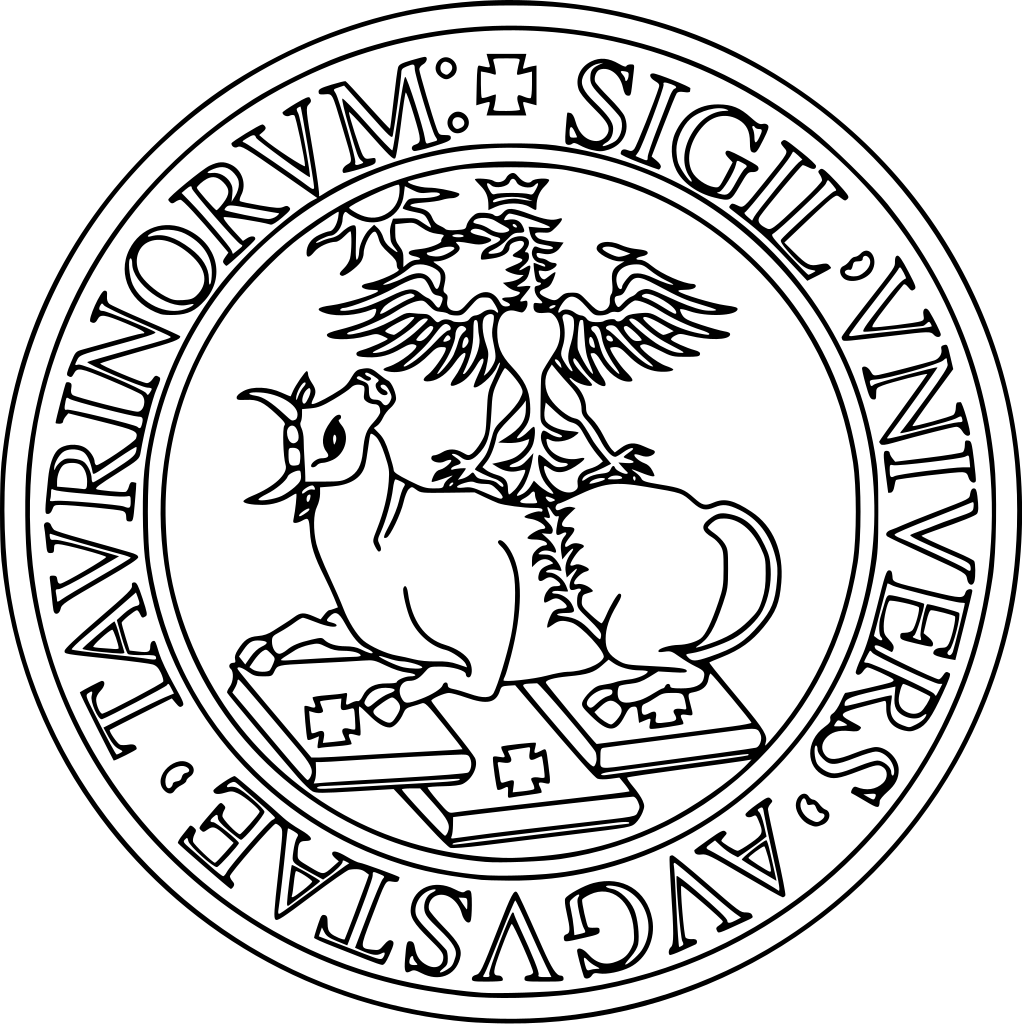
\includegraphics[width=10mm]{IMG/Unito.png}}
\usetheme{Madrid}
%\setbeamercovered{dynamic}
\setbeamertemplate{footline}[frame number]
\setbeamertemplate{navigation symbols}{}
\begin{document}
	
	\begin{frame}[noframenumbering]		
		\maketitle
	\end{frame}

	\begin{frame}[noframenumbering]
	\frametitle{Table of contents}
		\begin{columns}
			\column{0.3 \textwidth}
				\begin{center}
					\tableofcontents
				\end{center}
			\column{0.7 \textwidth}
				\begin{center}
					
\includegraphics[width=0.95 \textwidth]{IMG/Move_IT_logo.PNG}
				\end{center}
		\end{columns}
	\end{frame}

%%%%%%%%%%%%%%%%%%%%%%%%%%%%%%%%%%%%%%%%%%%%%%%%%%%%%%%%%%%%%%%%%%%%%%%%%%%%%%%%%%%%%%%%
	\section{Hadron therapy}
	
	\begin{frame}[plain, noframenumbering]
	%\frametitle{Hadron therapy, sensor and ASICs}
	\begin{center}
		{\Huge \fontfamily{qtm}\selectfont \color{blue} \textbf{Hadron therapy, sensor and ASICs}}
	\end{center}
	\end{frame}
	
	\begin{frame}
	\frametitle{Hadron therapy}
		\begin{columns}
		\column{0.40 \textwidth}
		\begin{center}
			\textbf{Hadron therapy} uses heavy charged particles (p, ${}^{12}$C ions) to administer a lethal dose to the tumor target minimizing the energy deposited in the surrounding healthy tissues.
			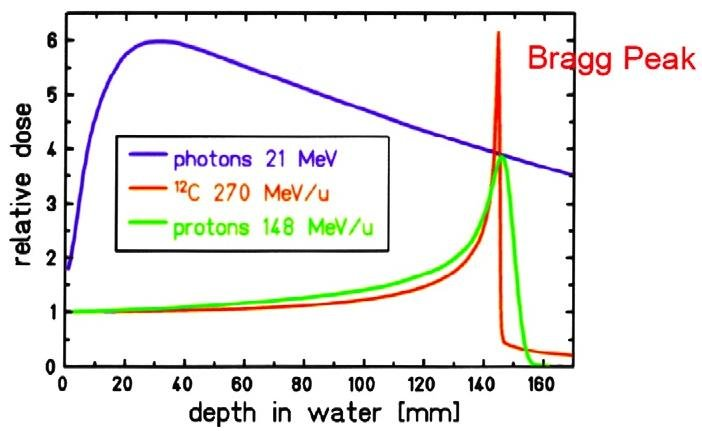
\includegraphics[width=0.95 \textwidth]{IMG/Bragg_Peak.PNG}
		\end{center}
		\column{0.60 \textwidth}
		
			{\color{blue} Advantages compared to x-ray radiotherapy:}
			\begin{itemize}
				\item Maximum dose delivered deep into tissue (Bragg peak)
				\item Greater conformation of the dose to the tumor
			\end{itemize}
		\vspace{1 cm}
			{\color{blue} Typical Proton Beam Parameters:}
			\begin{itemize}
				\item FWHM 3-7 mm
				\item Beam rates $10^6-10^{10}$ p/s
				\item Current  1-320 nA
				\item Energy  70-228 MeV
			\end{itemize}
		
		\end{columns}
	\end{frame}

	\begin{frame}
		\frametitle{Treatment Planning System (TPS)}
		\begin{columns}
			\column{0.5 \textwidth}
			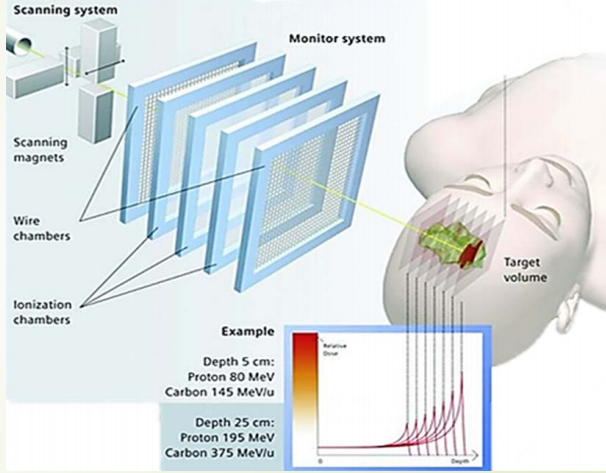
\includegraphics[width=0.95 \textwidth]{IMG/Beam_Monitoring.PNG}
			\column{0.5 \textwidth}
			\begin{itemize}
				\item Acquisition of morphological data by CT (\textbf{C}omputed \textbf{T}omography) and tumor volume identification
				\item Subdivision of the tumor into spots organized in layers of different depths corresponding to different beam energies
				\item Transverse scanning by deflecting the pencil beam via a pair of magnets
				\item Longitudinal scan by varying the energy of the beam
			\end{itemize}
		\end{columns}
	\vspace{0.2 cm}
	{\color{blue} Real-time beam detection parameters (direction and number of particles delivered) \newline is extremely important in order to distribute the dose accurately.}
	\end{frame}
	%I rivelatori controllano il trattamento, sulla base di queste informazioni viene controllata la posizione, la direzione e l'energia del fascio in tempo reale
	%Come si comportano dei rivelatori al silicio?

	\begin{frame}
		\frametitle{Beam monitoring}
		\begin{columns}
			\column{0.04 \textwidth}
			\column{0.2 \textwidth}
			\begin{center}
				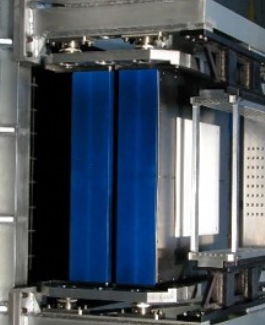
\includegraphics[width=0.95 \textwidth]{IMG/Ionization_Chamber.PNG}
			\end{center}
			\begin{center}
				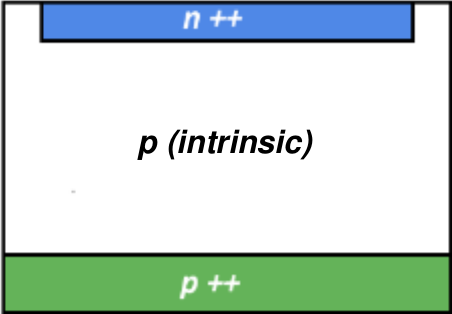
\includegraphics[width=0.95 \textwidth]{IMG/Solid_State_Detector.PNG}
			\end{center}
			\column{0.38 \textwidth}
			{\color{blue} Ionization chambers}
			\newline
			\textbf{Advantages}
			\begin{itemize}
				\item Structural integrity
				\item Radiation resistance
			\end{itemize}
			\textbf{Disadvantages}
			\begin{itemize}
				\item Slow response times $\approx 10^2\:\mu s$
				\item Limited sensitivity
				\item Indirect measurement of the number of particles
			\end{itemize}
			\column{0.38 \textwidth}
			{\color{blue} Solid state detectors}
			\newline
			\textbf{Advantages}
			\begin{itemize}
				\item Fast response times $\approx 1-2$ ns
				\item High spatio-temporal resolution
				\item Ideally, sensitive to the single particle
			\end{itemize}
			\textbf{Disadvantages}
			\begin{itemize}
				\item Complex and fast readout electronics
				\item Damage from radiation
			\end{itemize}
		\end{columns}
	\end{frame}


	
	\begin{frame}
	\frametitle{LGAD sensors}
	\begin{columns}
	\column{0.35 \textwidth}
		\begin{center}	
			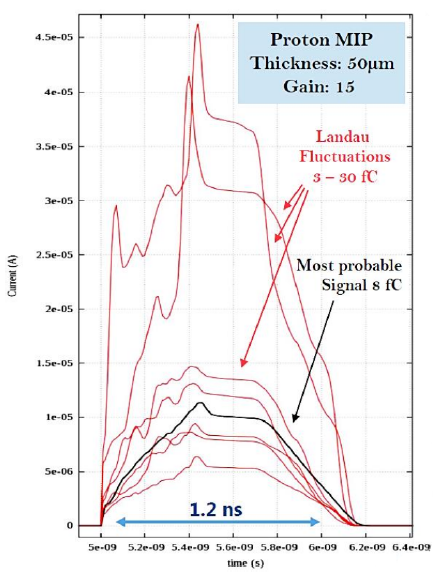
\includegraphics[width=0.9 \textwidth]{IMG/LGAD_Signal.PNG}
		\end{center}
	\column{0.65 \textwidth}
	\begin{center}
		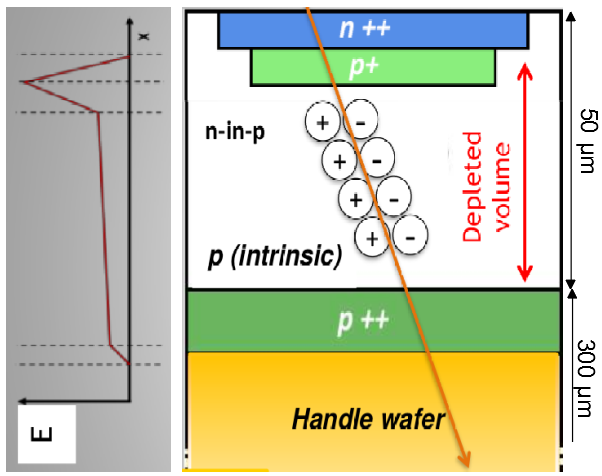
\includegraphics[width=0.4 \textwidth]{IMG/UFSDLGAD.PNG}
	\end{center}
		\begin{itemize}
			\item \textbf{L}ow \textbf{G}ain \textbf{A}valanche \textbf{D}etector
			\item 50$\mu$m sensor thickness
			\item Internal gain of \textbf{10-15} 
			\item Trapezoidal signal of $\approx$\textbf{1.5ns}\newline
				{\color{blue} Capable of detecting single particle }
			\item LGAD allows to increase SNR 
		\end{itemize}
	\end{columns}
	\end{frame}
	%mettere figura delle strip che usiamo noi
	%Per spessori piccoli il segnale è piccolo
	%Abbiamo bisogno di sensori piccoli perché la frequenza massima a cui possiamo contare dipende dalla durata del segnale
	%Servono spessori piccoli per avere segnali veloci 
	%Idealmente dovremmo usare i pixel
	%LGAD mi permette di aumentare il rapporto segnale-su-rumore
	%Aggiungere segnale dell'LGAD


	\begin{frame}
	\frametitle{ABACUS\_v2}
	\begin{columns}
		\column{0.25 \textwidth}
		\begin{center}
				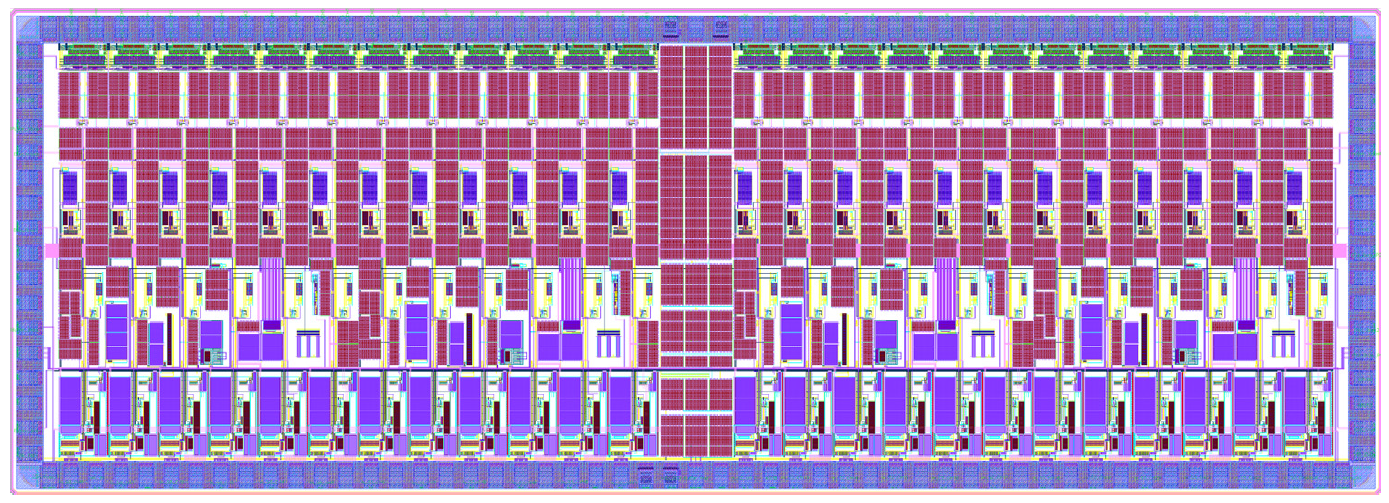
\includegraphics[width=1.85 \textwidth, angle=90]{IMG/ABACUS.PNG}
		\end{center}
		\column{0.75 \textwidth}
		\begin{center}
			{\color{blue} \textbf{ABACUS\_v2}}={\tiny \textbf{A}synchronous-logic-\textbf{B}ased \textbf{A}nalog \textbf{C}ounter for \textbf{U}ltra fast \textbf{S}ilicon strips}
		\end{center}
		\begin{columns}
			\column{0.5 \textwidth}
			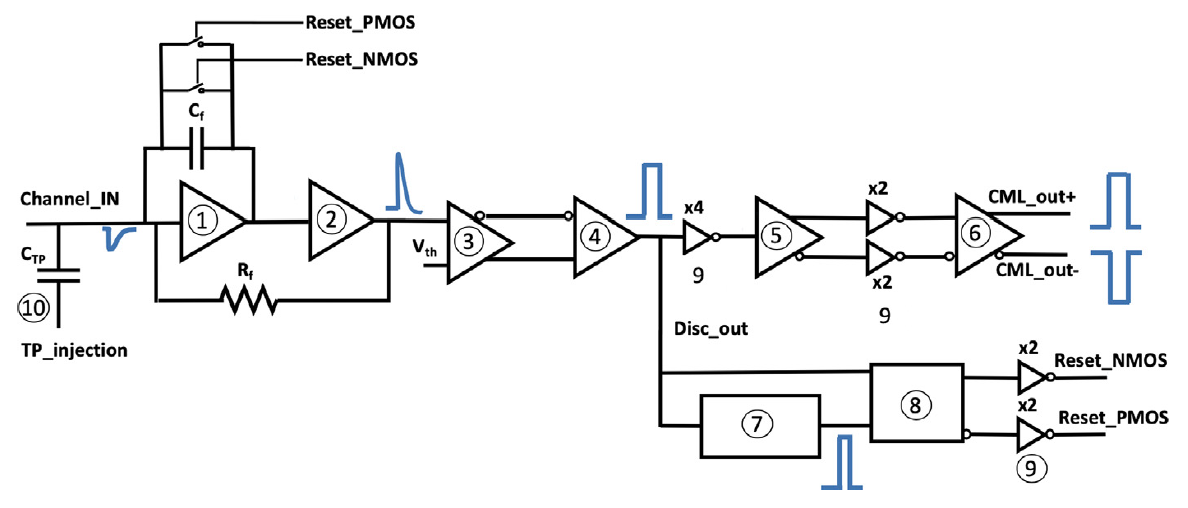
\includegraphics[width=0.99 \textwidth]{IMG/ABACUS_channel.PNG}
			\column{0.5 \textwidth}
			\begin{itemize}
				\item 110 nm technology
				\item 24 channels
				\item I2C controller for digital configuration
				\item Die size 4.95 x 1.935 mm$^2$
				%Dead time <10ns
				%SNR>10
				%possibilità di simulare segnali mandando impulsi su canali pari o dispari
				%range di carica in ingresso 3fC-140fC
			\end{itemize}
		\end{columns}
		{\color{blue} Channel structure }
		\begin{itemize}
			\item Charge sensitive amplifier
			\item Discriminator controlled by two DACs
			\begin{itemize}
				\item External DAC (common for all channel)
				\item Programmable internal DAC (6 bit) for each channel
			\end{itemize}
			\item Fast reset signal to discharge capacitive feedback
		\item CML converter  
		\end{itemize} 
	\end{columns}
	\end{frame}

		\begin{frame}
	\frametitle{ABACUS\_v2 internal DACs setup}	
	\begin{columns}
		\column{0.5 \textwidth}
		\begin{center}
			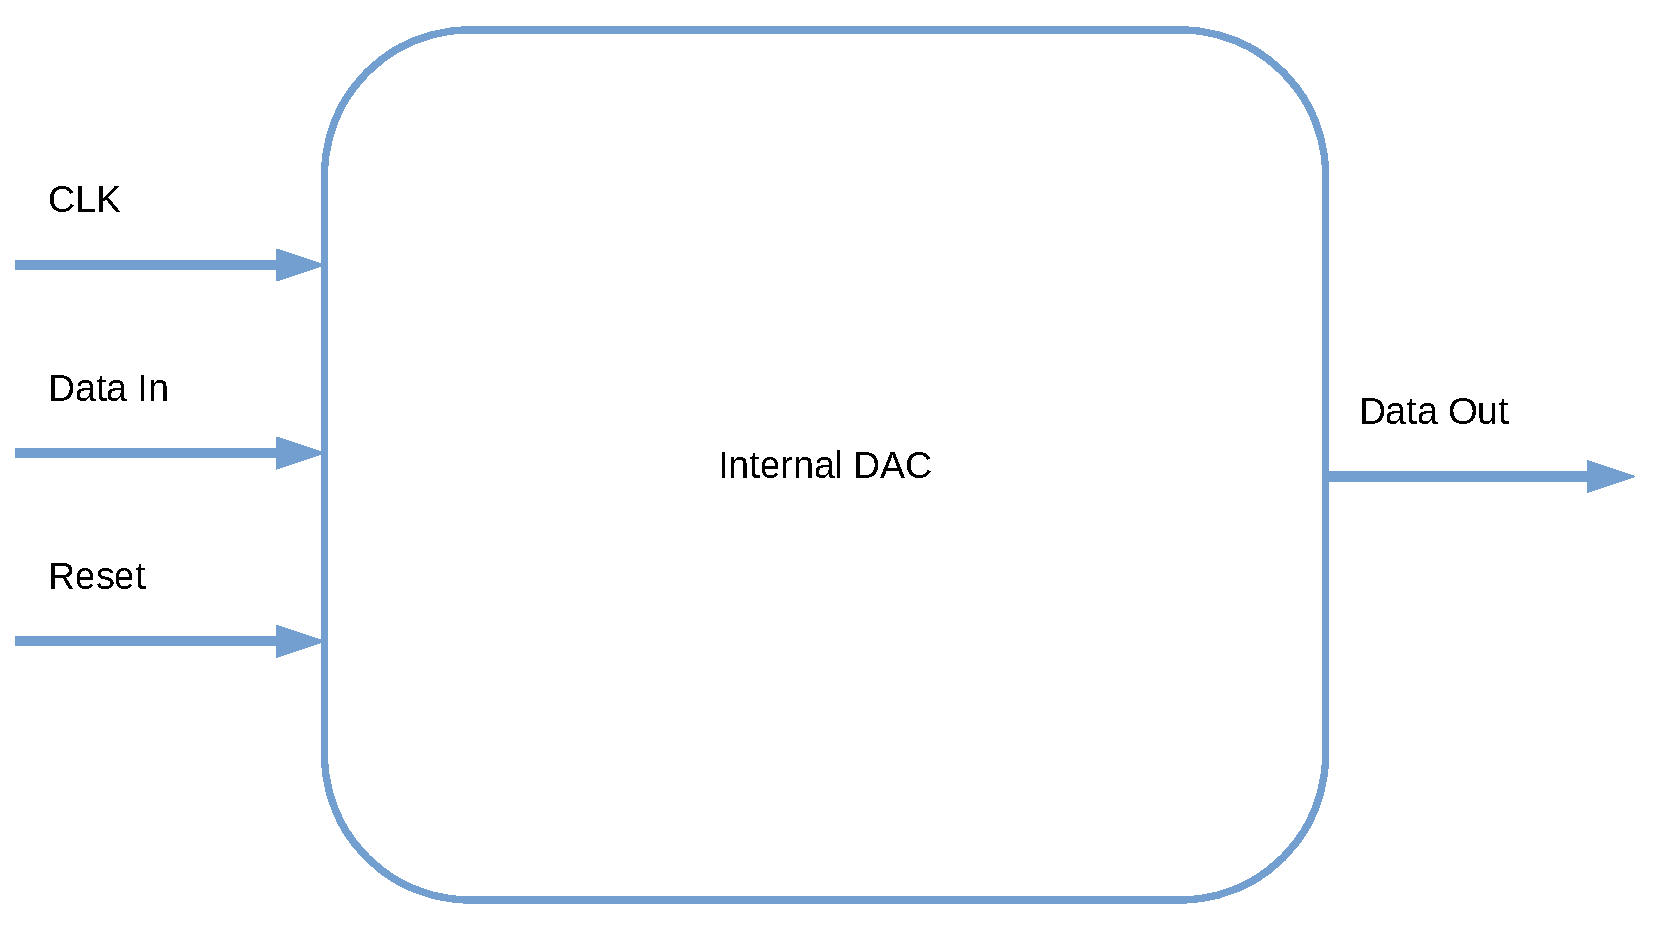
\includegraphics[width=0.7 \textwidth]{IMG/InternalDAC.pdf}
			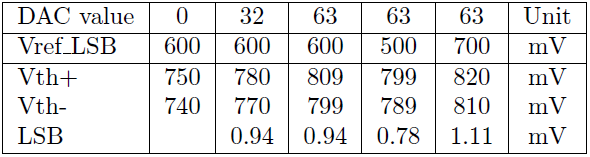
\includegraphics[width=0.7 \textwidth]{IMG/TableLSB.PNG}
		\end{center}
		\textbf{LSB} value $\approx$0.94 mV for \textbf{Vref\_LSB}=600 mV
		\column{0.5 \textwidth}
		{\color{blue} Internal DAC setup}
		\begin{itemize}
			\item Initialization sequence \textbf{A5A5}= 
			\newline
			1010-0101-1010-0101
			\item \textbf{16bit words}= \newline 2bit command + 6bit address + 8bit data
			\begin{itemize}
				\item \textbf{command}
				\begin{itemize}
					\item \textbf{11} = write
					\item \textbf{10} = read
				\end{itemize}
				\item \textbf{address}
				\begin{itemize}
					\item \textbf{5bit} address from \textbf{0} to \textbf{23}
					\item \textbf{LSB} is Vth+- (not used for now)
				\end{itemize}
				\item \textbf{data}
				\begin{itemize}
					\item \textbf{2MSB} not used
					\item \textbf{6LSB} data for the internal DAC \newline from \textbf{0} to \textbf{63}
				\end{itemize}
			\end{itemize} 
		\end{itemize}
	\end{columns}
	\end{frame}

		\begin{frame}
	\frametitle{FPGA}
	\begin{center}
		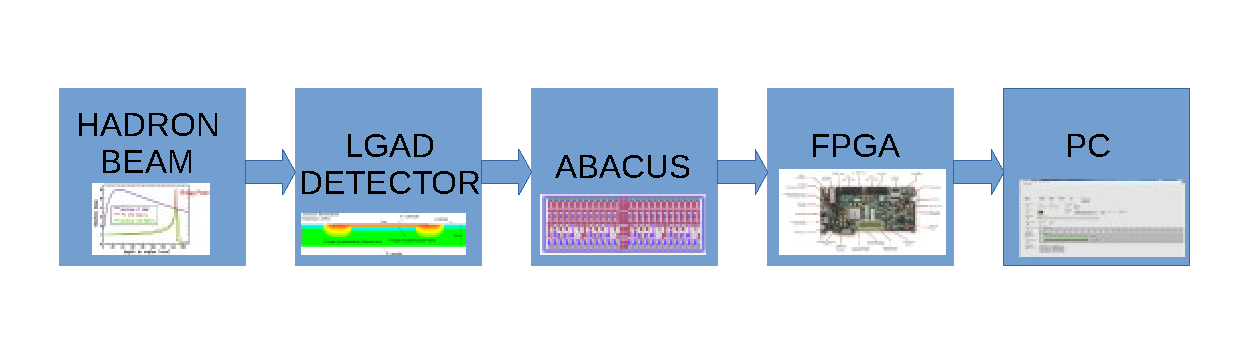
\includegraphics[width=0.7 \textwidth]{IMG/Block_Diagram.pdf}
	\end{center}
		\begin{itemize}
			\item FPGA = \textbf{F}ield \textbf{P}rogrammable \textbf{G}ate \textbf{A}rray
			\begin{itemize}
				\item Gate array : \textbf{array of "logic cells"} that can be programmed to implement \textbf{any desired logic functionality}
				\item Field programmable: \textbf{device not committed to do something} until effectively programmed according to the field application
			\end{itemize}
			\item In principle, \textbf{programmable infinite times} with no limitations
			\item \textbf{High flexibility}: it can be implemented \textbf{any digital function}
			\item \textbf{Fast} and \textbf{cheap} prototyping: \textbf{out of the box} solution: no layout or masks
			\item {\color{orange} Power hungry, slow compared to \textbf{ASICs} and expensive on large-scales}
		\end{itemize}
	\end{frame}

\section{Move\_IT}

	\begin{frame}
	\frametitle{MoVe\_IT project}
	\begin{center}
		{\color{blue} MoVe\_IT = \textbf{Mo}deling and \textbf{Ve}rification for \textbf{I}on beam \textbf{T}reatment planning }
		\newline
		Prove the ability of LGAD detectors to discriminate individual protons and to count their number up to fluxes of 100 MHz / cm2 with an uncertainty of {\color{blue}less than 1\%}, (clinical tolerance required)
	\end{center}
	\begin{columns}
		\column{0.6 \textwidth}
		\begin{itemize}
			\item Single proton counting:
			\item Area 3x3 cm${}^2$ with 144 Strips;
			\item Max rates= $10^8$ p/s cm2 ({\color{blue} Error < 1\%})
			\item Two orthogonal directions
		\end{itemize}
		\column{0.4 \textwidth}
		\begin{center}
			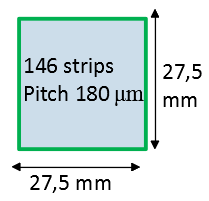
\includegraphics[width=0.7 \textwidth]{IMG/Detector.PNG}
		\end{center}
	\end{columns}
	\end{frame}
	
%%%%%%%%%%%%%%%%%%%%%%%%%%%%%%%%%%%%%%%%%%%%%%%%%%%%%%%%%%%%%%%%%%%%%%%%%%%%%%%%%%%%%%%%
\section{Experimental setup}

\begin{frame}[plain, noframenumbering]
\begin{center}
	{\Huge \fontfamily{qtm}\selectfont \color{blue} \textbf{Experimental setup}}
\end{center}
\end{frame}



	\begin{frame}
	\frametitle{Test board}
		\begin{columns}
			\column{0.5 \textwidth}
			\begin{center}
				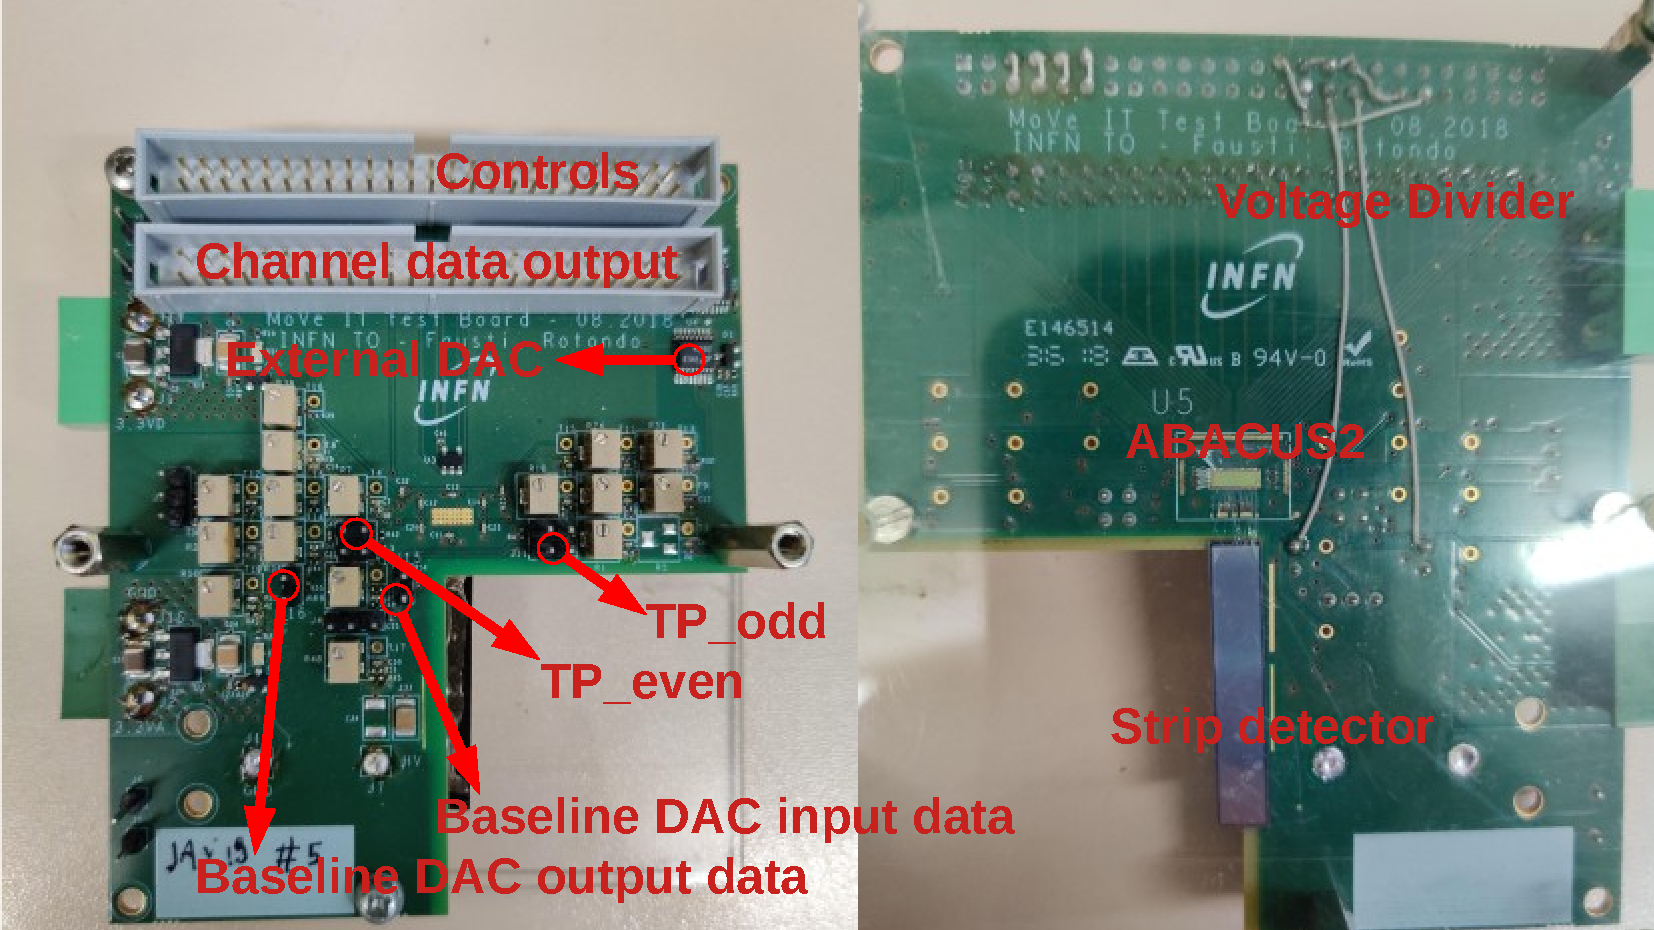
\includegraphics[width=0.8 \textwidth]{IMG/TestBoard.pdf}
				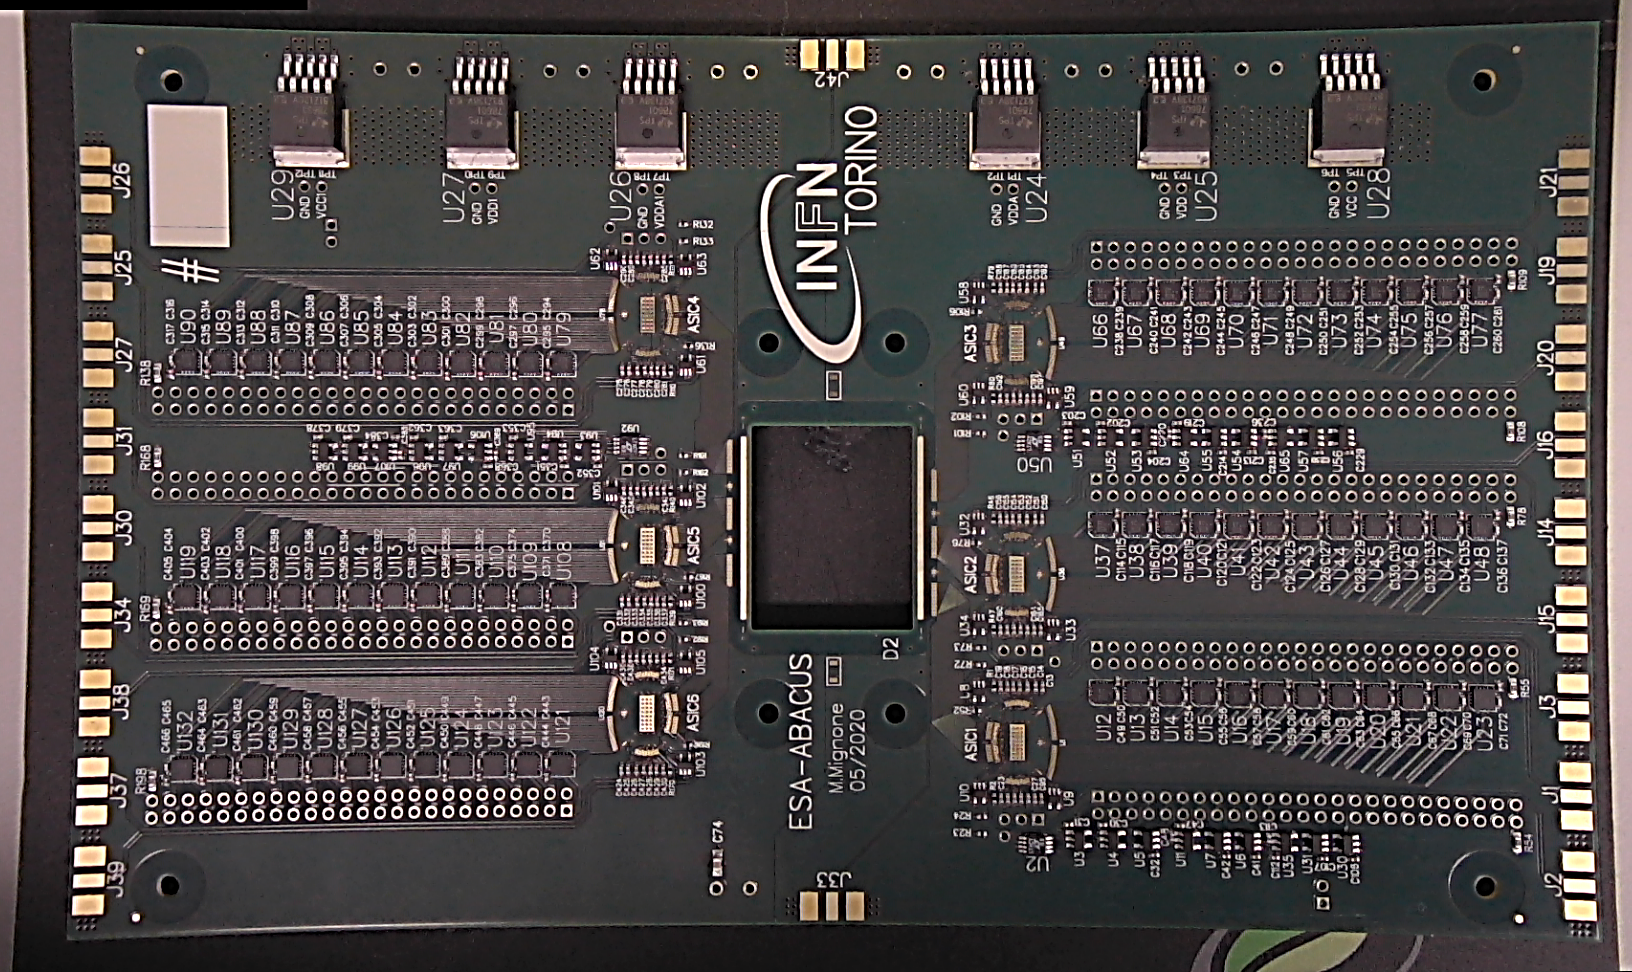
\includegraphics[width=0.8 \textwidth]{IMG/EsaAbacus.png}
			\end{center}
			\column{0.5 \textwidth}
			{\color{blue}ABACUS\_v2 test board}
			\begin{itemize}
				\item 1 ABACUS ASIC chip
				\item CML output to FPGA
				\item I2C input to internal DACs
				\item \textbf{TP\_even} and \textbf{TP\_odd}
			\end{itemize}
			{\color{blue}Esa-ABACUS}
			\begin{itemize}
				\item 6 ABACUS chips
				\item Able to read 144 strips
				\item 3 FPGA needed
			\end{itemize}
		\end{columns}	
	\end{frame}

	\begin{frame}
	\frametitle{Experimental setup}
		\begin{columns}
			\column{0.65 \textwidth}
			\begin{center}
				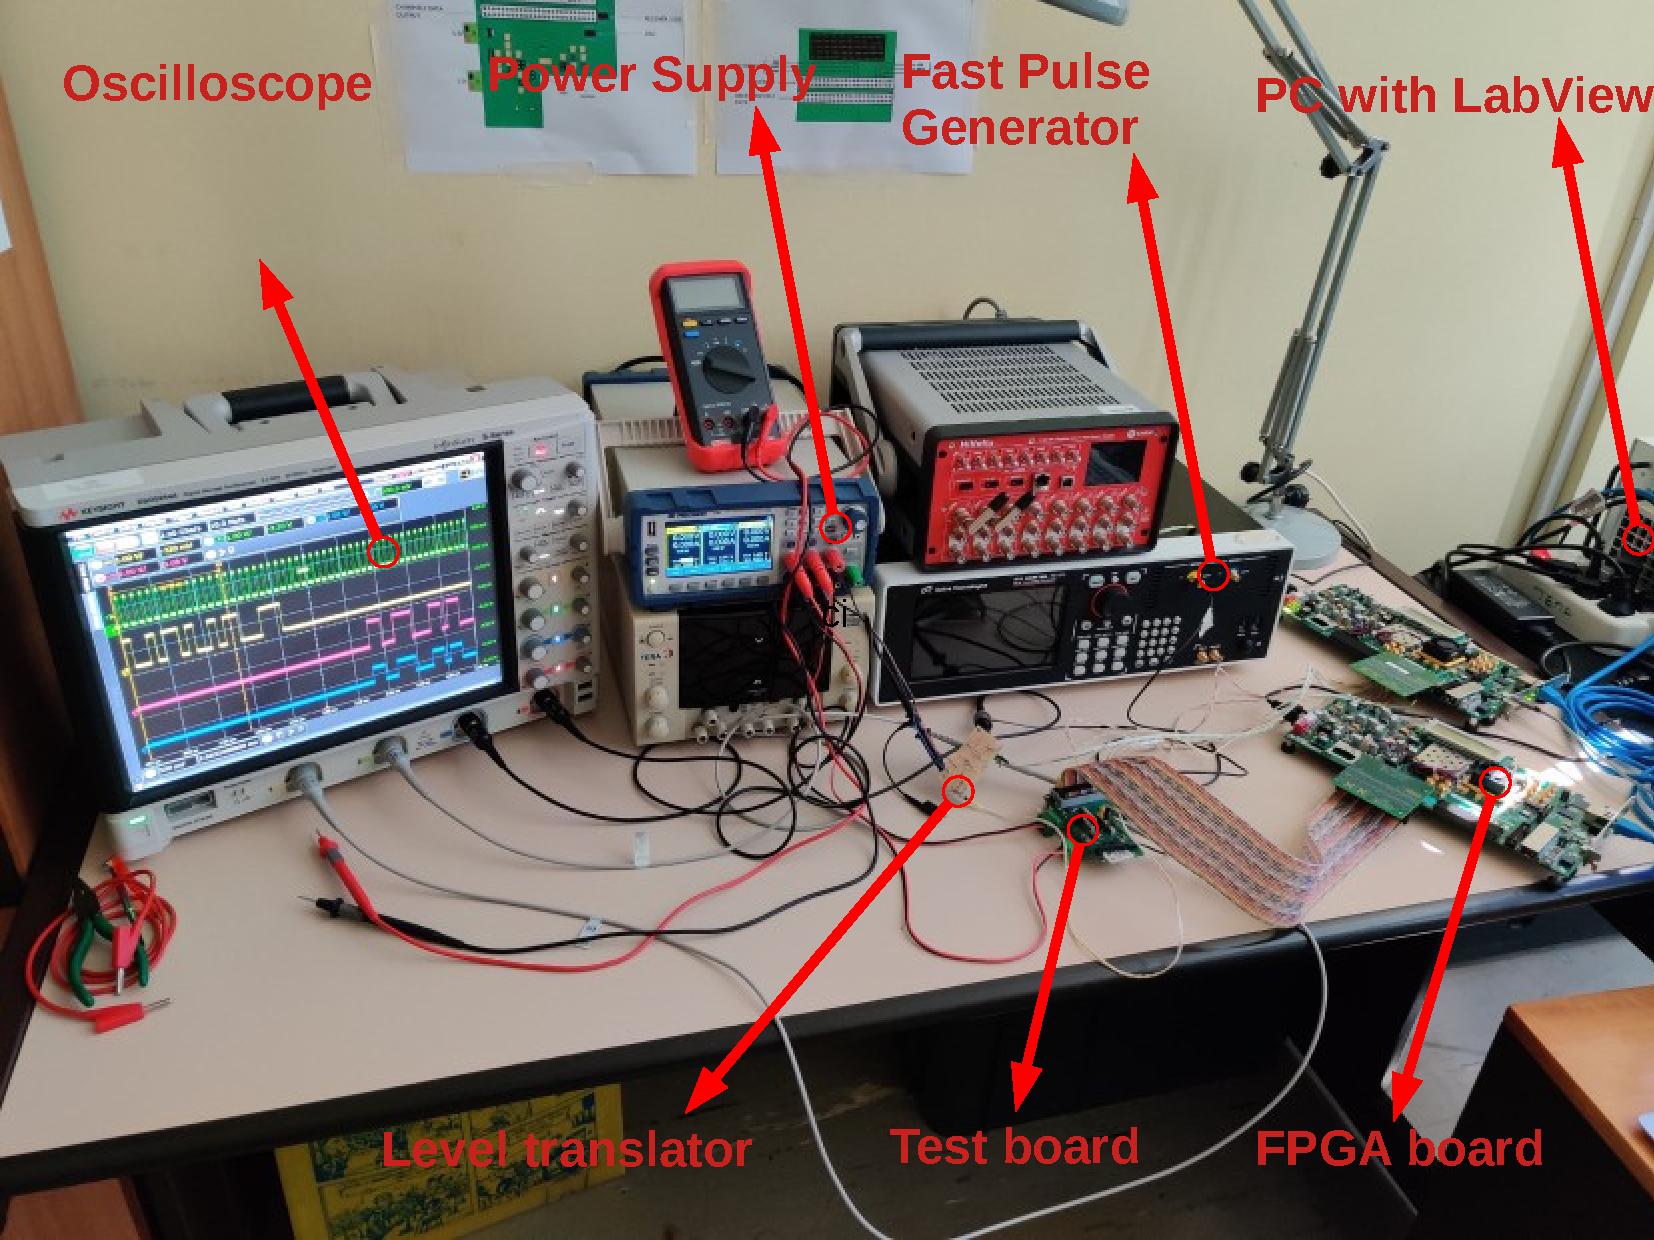
\includegraphics[width=0.95 \textwidth]{IMG/TestBench.pdf}
			\end{center}
			\column{0.35 \textwidth}
			\begin{itemize}
				\item Impulsator
				\item Oscilloscope
				\item Power Supply
				\item FPGA
				\item Test Board
				\item PC
			\end{itemize}
		\end{columns}
		
	\end{frame}


%%%%%%%%%%%%%%%%%%%%%%%%%%%%%%%%%%%%%%%%%%%%%%%%%%%%%%%%%%%%%%%%%%%%%%%%%%%%%%%%%%%%%%%%

	\section{Personal Contribution}
	
	\begin{frame}[plain, noframenumbering]
		\begin{center}
			{\Huge \fontfamily{qtm}\selectfont \color{blue} \textbf{Personal contribution to the project}}
		\end{center}
	\end{frame}
	
	
	\begin{frame}
	\frametitle{Personal Contribution}
	\begin{itemize}
		\item {\color{green} Creation of a \textbf{debug} tool for the FMC connectors}
		\item {\color{green} Firmware implementation of the read/write logic for the \textbf{ABACUS} chip}
		\item {\color{green} Creation of the level translation device for communication with the \textbf{FPGA}}
		\item {\color{orange} Addition of a \textbf{latch} in order to save into a \textbf{register} the current state of every counter}
		\item {\color{orange} Addition of a \textbf{timestamp} in order to obtain a more accurate rate calculation}
		\item {\color{orange} Addition of a configurable \textbf{mask} to calculate via firmware the \textbf{sum} of only certain selected channels}
	\end{itemize}
	\end{frame}
	
	\begin{frame}
		\frametitle{Debug Tool}
		\begin{columns}
			\column{0.5 \textwidth}
			\begin{center}
				{\color{blue} KINTEX7 KC705}
				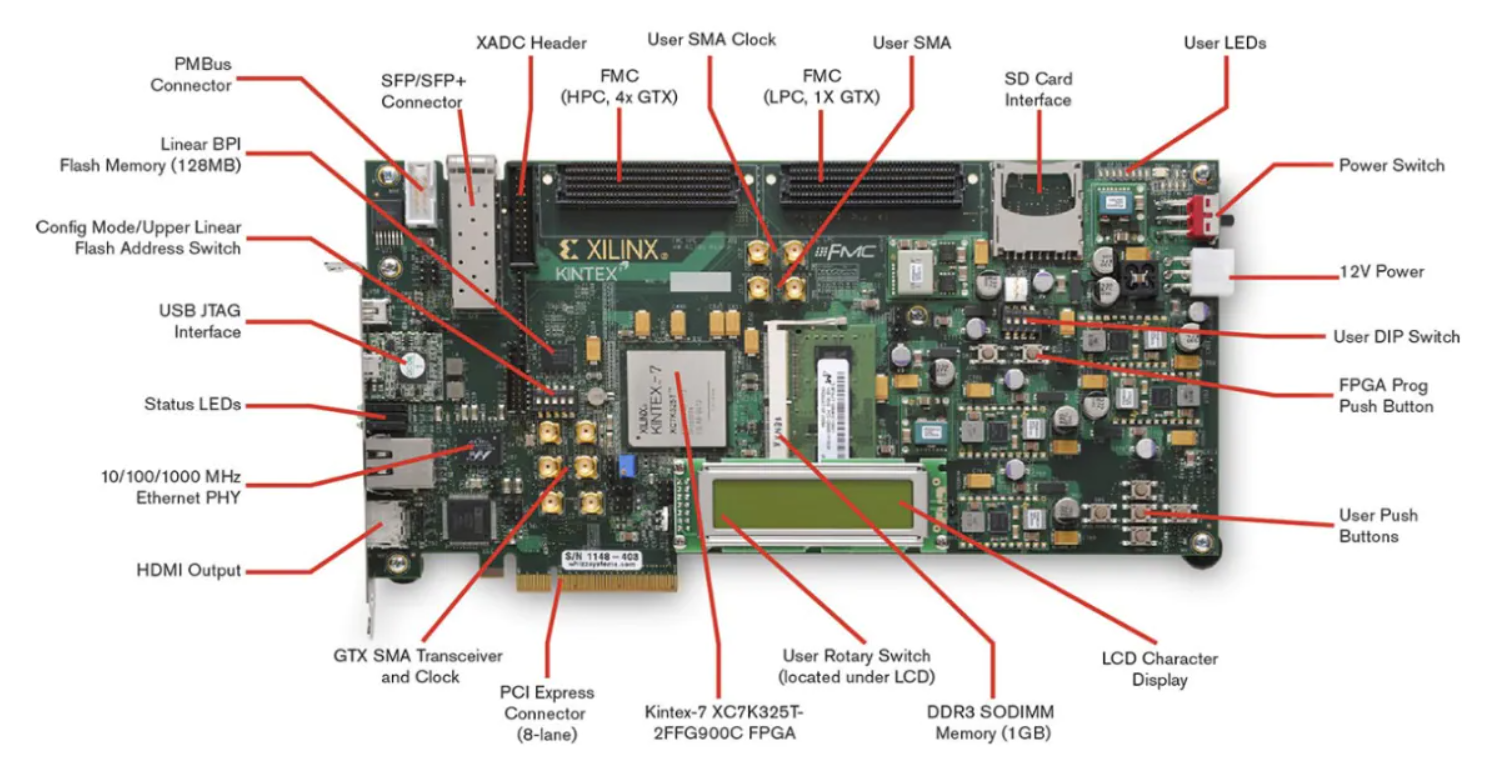
\includegraphics[width=1.0 \textwidth]{IMG/KC705.PNG}
			\end{center}
			\column{0.5 \textwidth}
			\textbf{FMC} connector
			\begin{itemize}
				\item \textbf{LPC}= \textbf{L}ow \textbf{P}in \textbf{C}ount
				\item \textbf{HPC}= \textbf{H}igh \textbf{P}in \textbf{C}ount
				\item \textbf{LVDS} output 
			\end{itemize}
			\textbf{Debug}
			\begin{itemize}
				\item Set every pin as an \textbf{output}
				\item Switch state with a button
				\item Measure voltages with multimeter
			\end{itemize}
		\end{columns}
	\end{frame}

	\begin{frame}
	\frametitle{Level translator}
	\begin{columns}
		\column{0.35 \textwidth}
		\begin{center}
			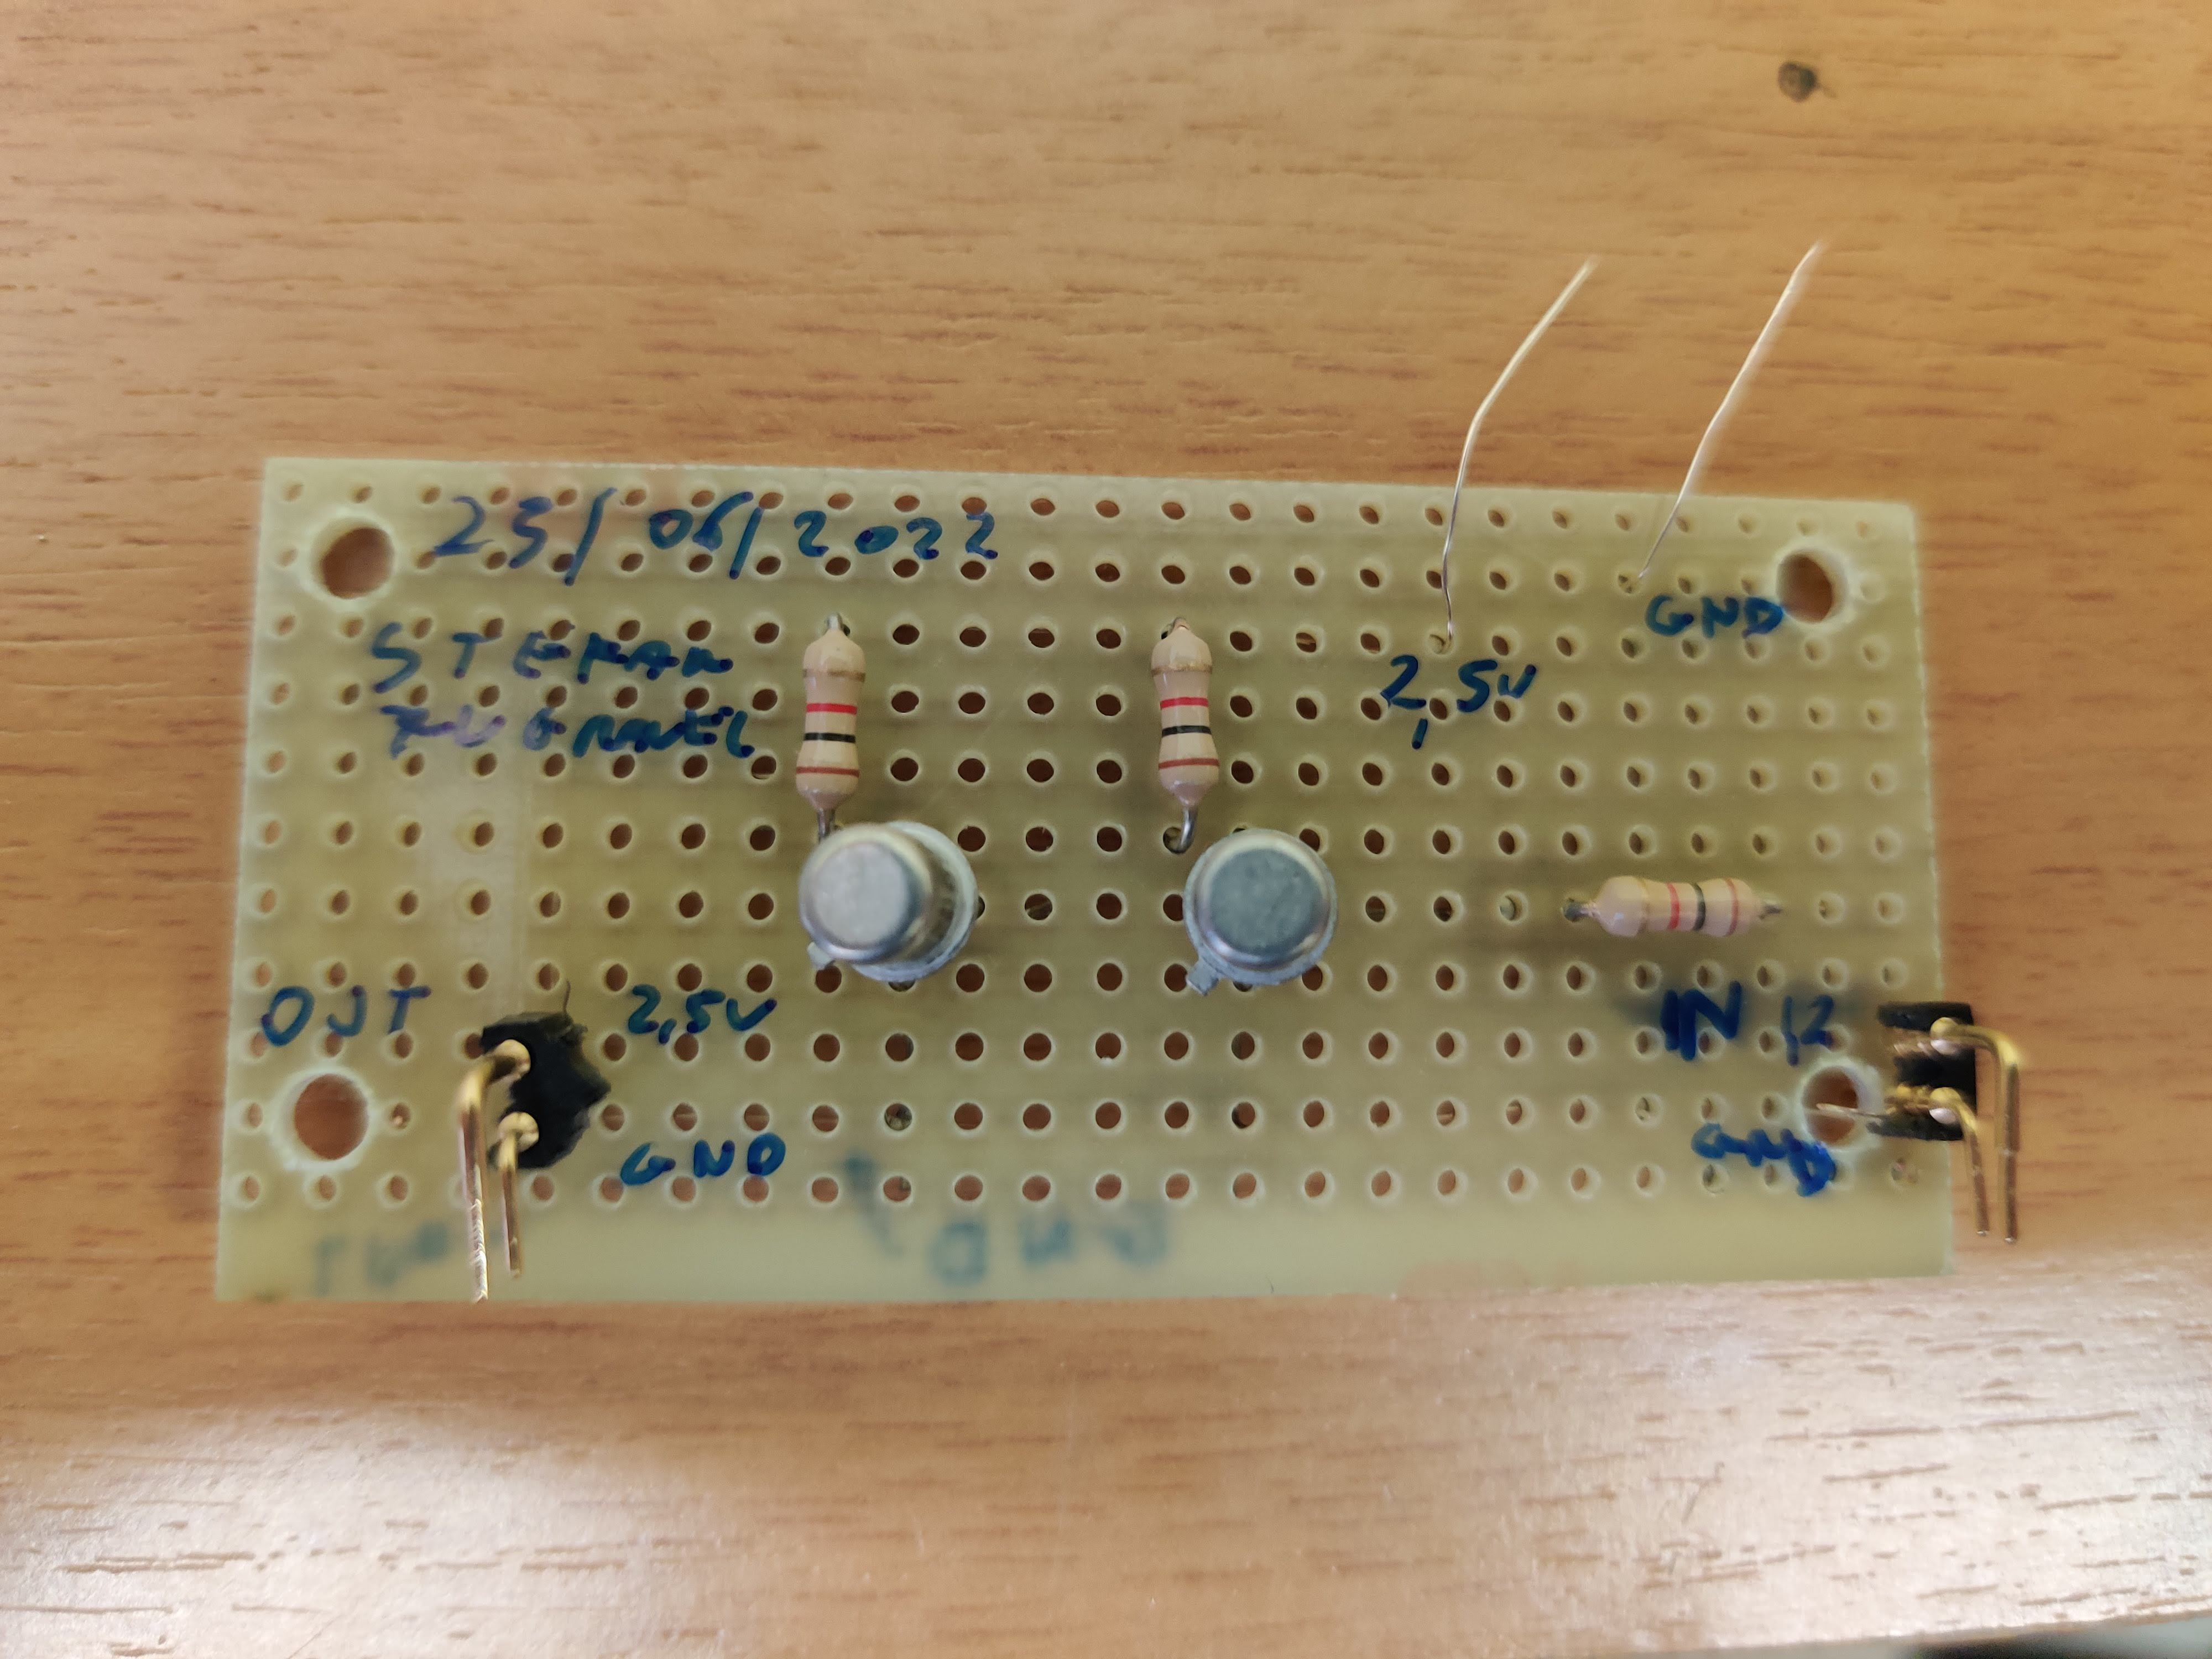
\includegraphics[width=0.8 \textwidth]{IMG/level_translator_front-min.jpg}
			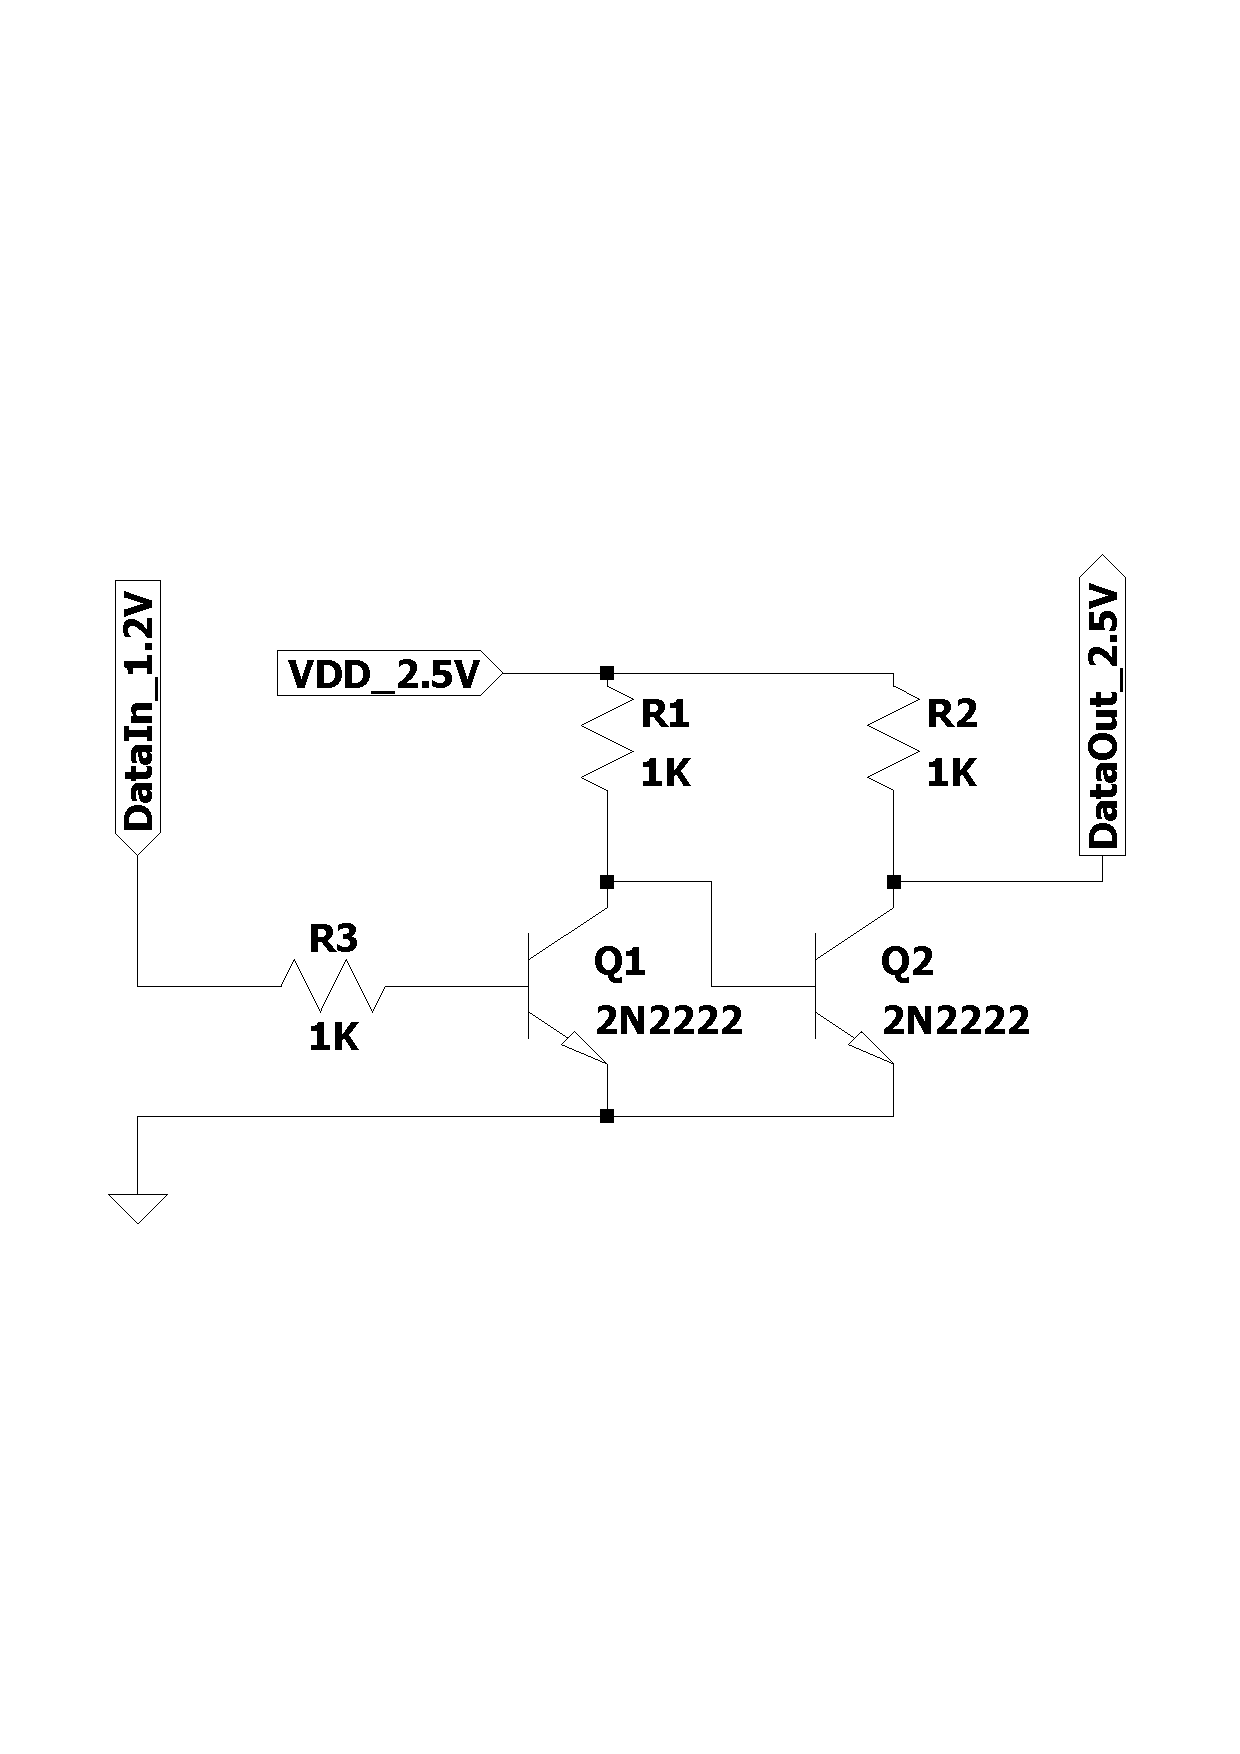
\includegraphics[width=0.8 \textwidth]{IMG/Diagram_cropped.pdf}
		\end{center}
		\column{0.65 \textwidth}
		\begin{itemize}
			\item ABACUS output = \textbf{1.2}V single-ended
			\item FPGA input = \textbf{2.5}V single-ended
			\item 2x \textbf{2N2222} NPN transistor in TO-18 package
			\item 3x \textbf{1}k$\Omega$ resistor 1/8W
			\item 2x connectors \& wire
		\end{itemize}
		\begin{center}
			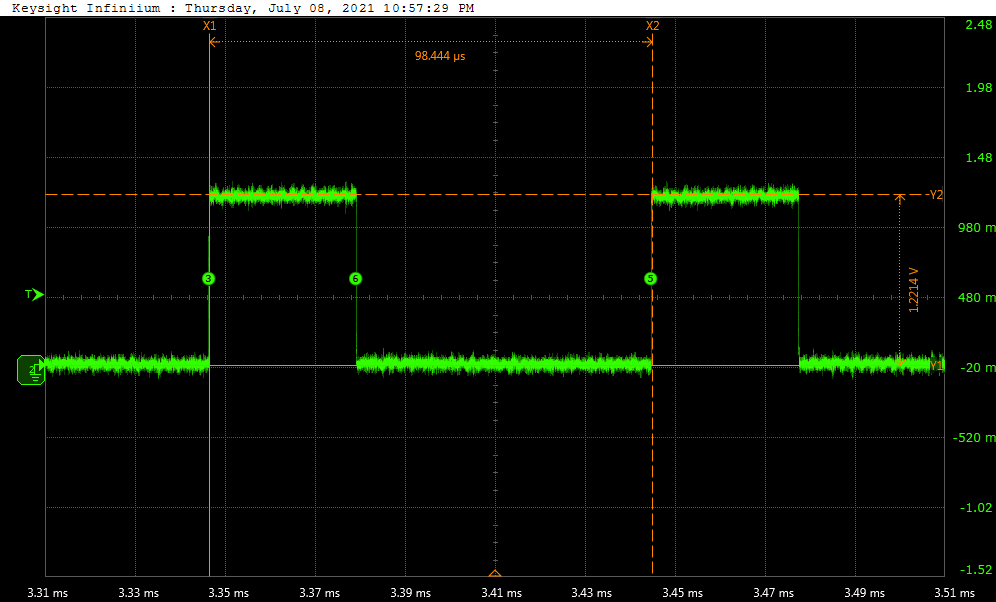
\includegraphics[width=0.5 \textwidth]{IMG/probe/09-08-2021_clock-specks.png}
		\end{center}
	\end{columns}
	\end{frame}

	\begin{frame}
		\frametitle{Firmware}
		\begin{columns}
			\column{0.5 \textwidth}
			\begin{center}
				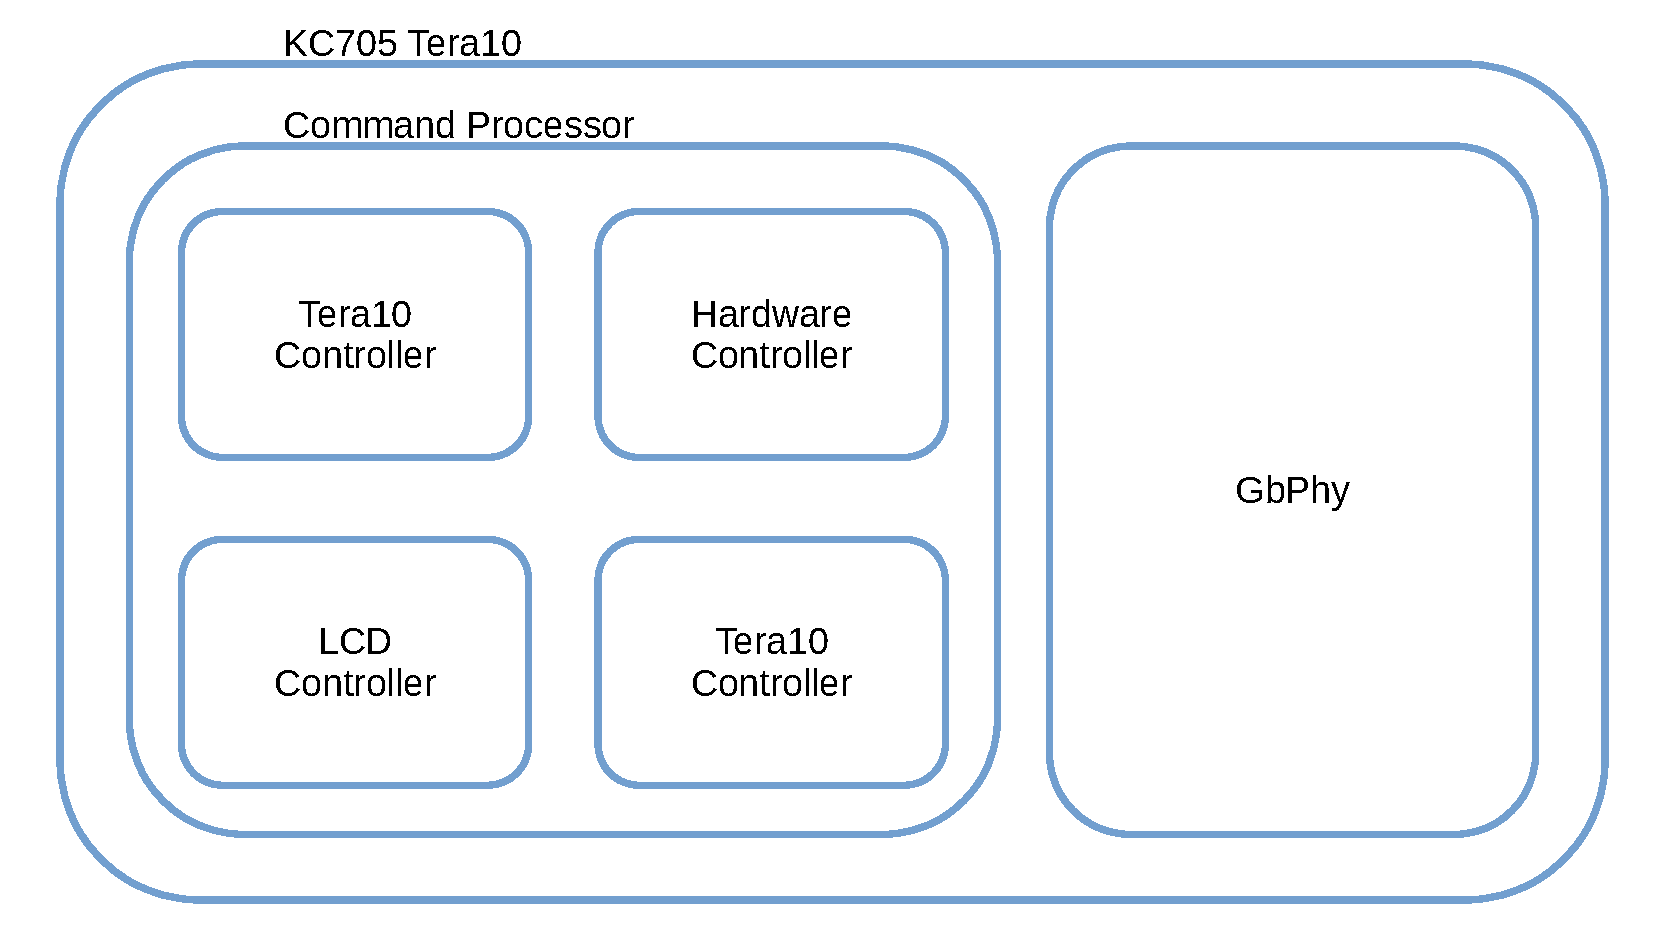
\includegraphics[width=1.0 \textwidth]{IMG/Tera10kc705.pdf}
			\end{center}
			\column{0.5 \textwidth}
			\begin{itemize}
				\item GbPhy = Custom \textbf{UDP} Protocol
				\item LCD Controller = display informations
				\item Tera10 IO = Input setup and counters
				\item Tera10 controller
				\item Hardware controller = setup internal and external Dacs
			\end{itemize}
		\end{columns}
	\end{frame}


	\begin{frame}
	\frametitle{Firmware - DATA}
	\begin{itemize}
		\item The \textbf{FPGA} communicates with the pc using UDP (\textbf{U}ser \textbf{D}atagram \textbf{P}rotocol) implemented in the \textbf{GbPhy} project
		\item Each UDP packet is \textbf{64} bit long $\rightarrow$ \textbf{32} bit used by GbPhy and \textbf{32} bit of data
		\item \textbf{32} bit data =
		\begin{itemize}
			\item \textbf{4} bit $\rightarrow$ firmware target
			\item \textbf{8} bit $\rightarrow$ firmware command
			\item \textbf{20} bit $\rightarrow$ firmware data
		\end{itemize}
		\item \textbf{20} bit firmware data =
		\begin{itemize}
			\item \textbf{3} bit not used
			\item \textbf{2} bit baseline dac command
			\item \textbf{6} bit baseline dac address
			\item \textbf{8} bit baseline dac data
			\item \textbf{1} bit baseline dac selecet (each FPGA can control 2 chips)
		\end{itemize}
		\item To perform a Read/write operation the initialization sequence must be sent first\newline every time
	\end{itemize}
	\end{frame}

	\begin{frame}[fragile]
		\frametitle{Firmware - FSM}
		\begin{itemize}
			\item FSM (\textbf{F}inite \textbf{S}tate \textbf{M}achine): states for the serial data communication
		\end{itemize}
		\begin{center}
			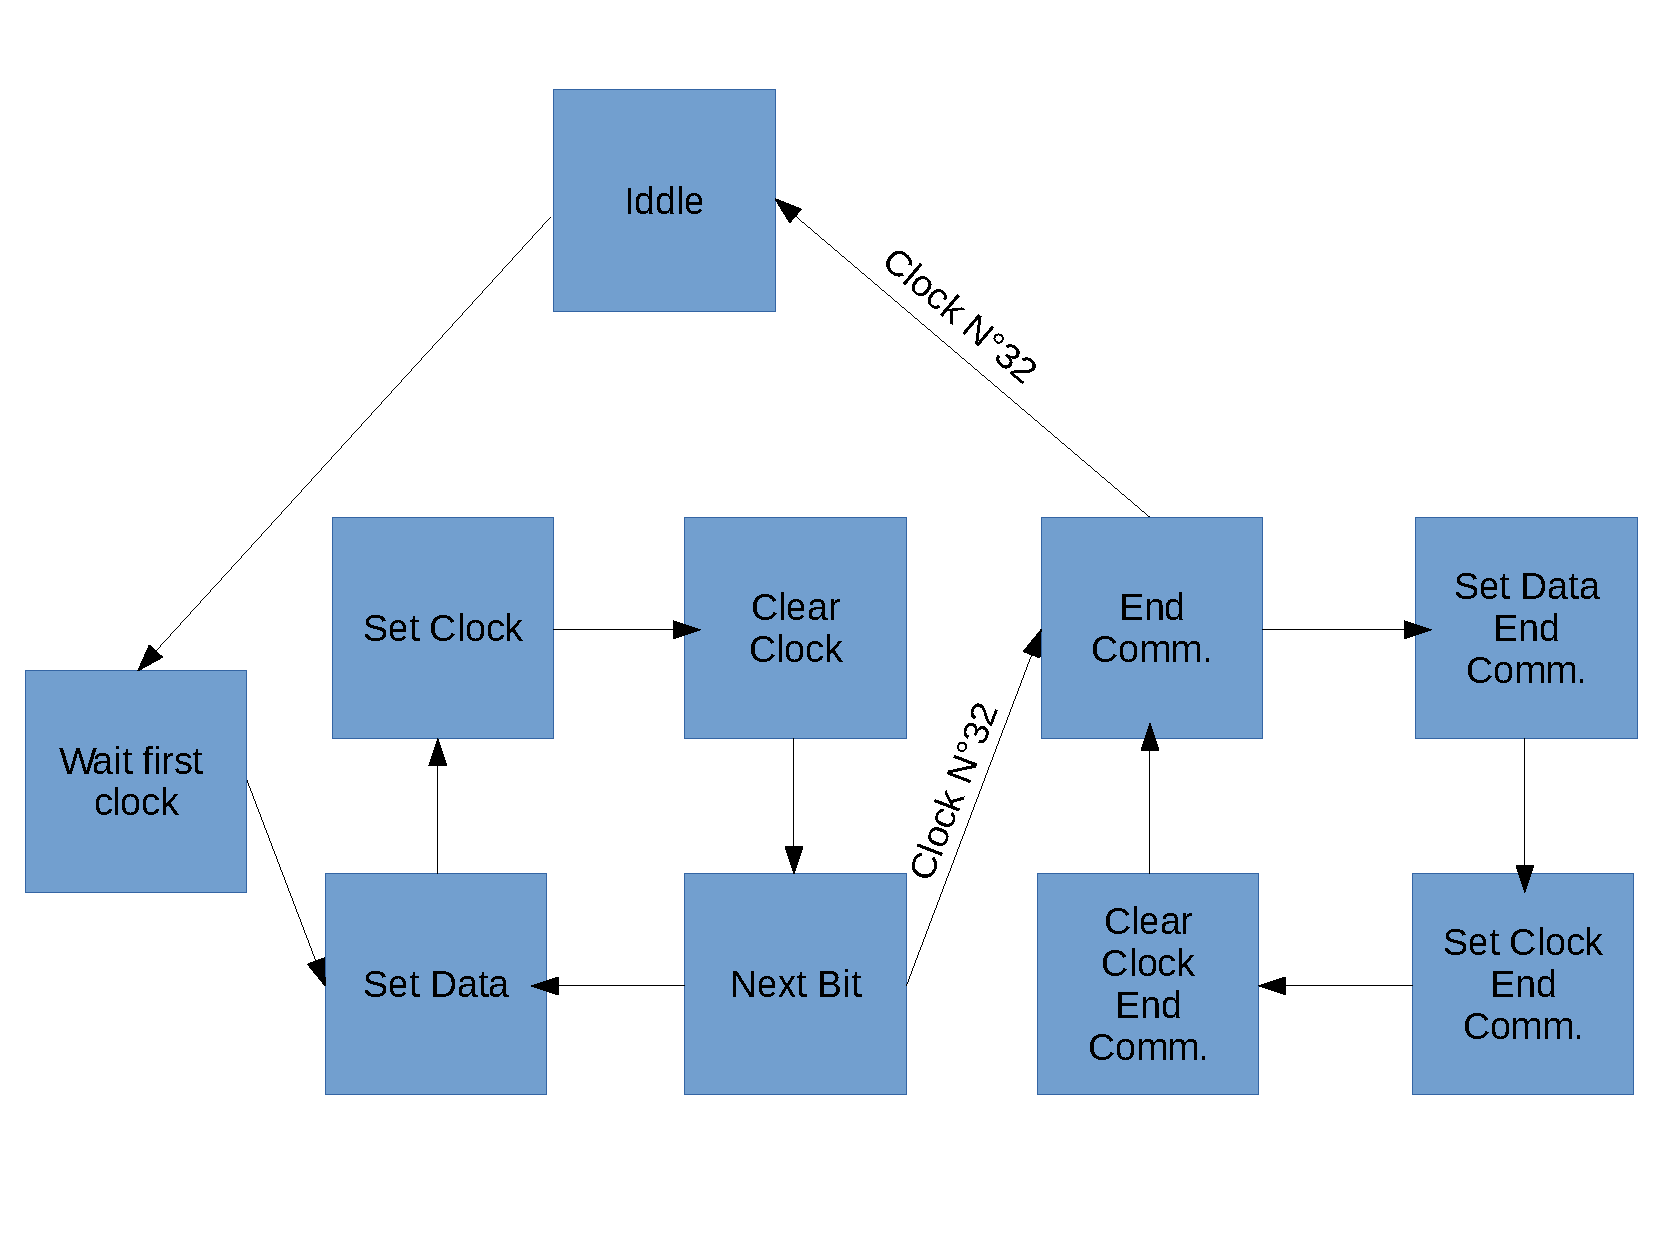
\includegraphics[width=0.45 \textwidth]{IMG/FSM.pdf}
		\end{center}
	\end{frame}


	\begin{frame}
	\frametitle{Vivado simulation}
		\begin{center}
			Finite State Machine
			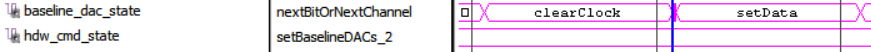
\includegraphics[width=0.9 \textwidth]{IMG/Simulation1.png}
			\newline
			write internal DAC channel 4
			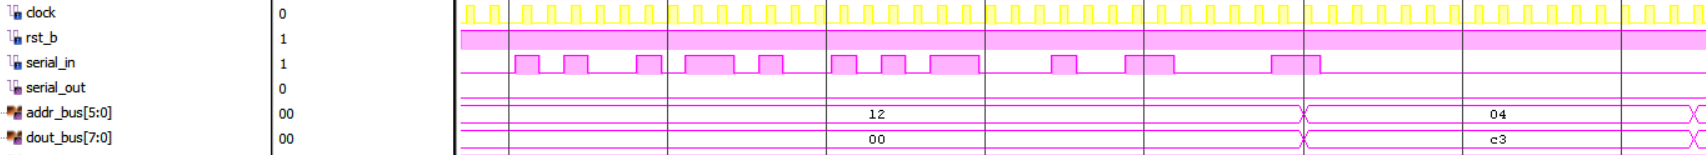
\includegraphics[width=0.9 \textwidth]{IMG/Simulation3.png}
			\newline
			read internal DAC channel 4
			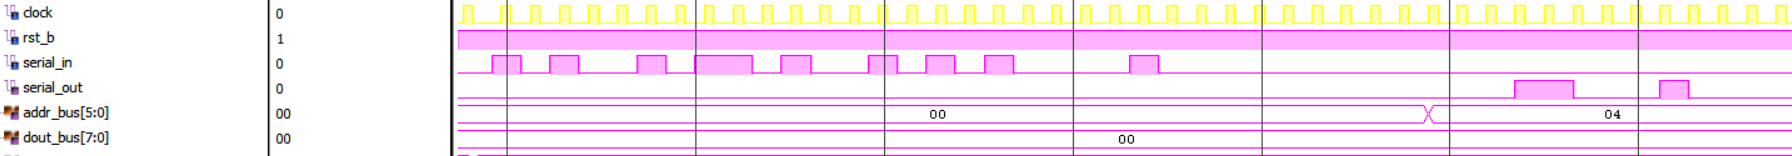
\includegraphics[width=0.9 \textwidth]{IMG/Simulation4.png}
		\end{center}
	The DAC behaviour is simulated by a Verilog module
	\end{frame}

	
	\begin{frame}
	\frametitle{Writing Baseline DACs}
	\begin{columns}
		\column{0.5 \textwidth}
	{\color{blue} Input}
	\begin{itemize}
		\item Initialization sequence = A5A5
		\item Command = 11 = write
		\item Address = 100010 = 10001-0 = channel 17
		\item Data    = 00111111 = 63
	\end{itemize}
	\column{0.5 \textwidth}
	{\color{blue} Clock Stats}
	\begin{itemize}
		\item Period = \textbf{98.44} $\mu$s
		\item Duty cycle \textbf{33}\%
		\item Packet duration $\approx$ \textbf{6.4} ms
	\end{itemize}
	\end{columns}
	\begin{center}
		{\color{green} clock signal}
		{\color{yellow} input data}
	\end{center}
	\begin{center}
		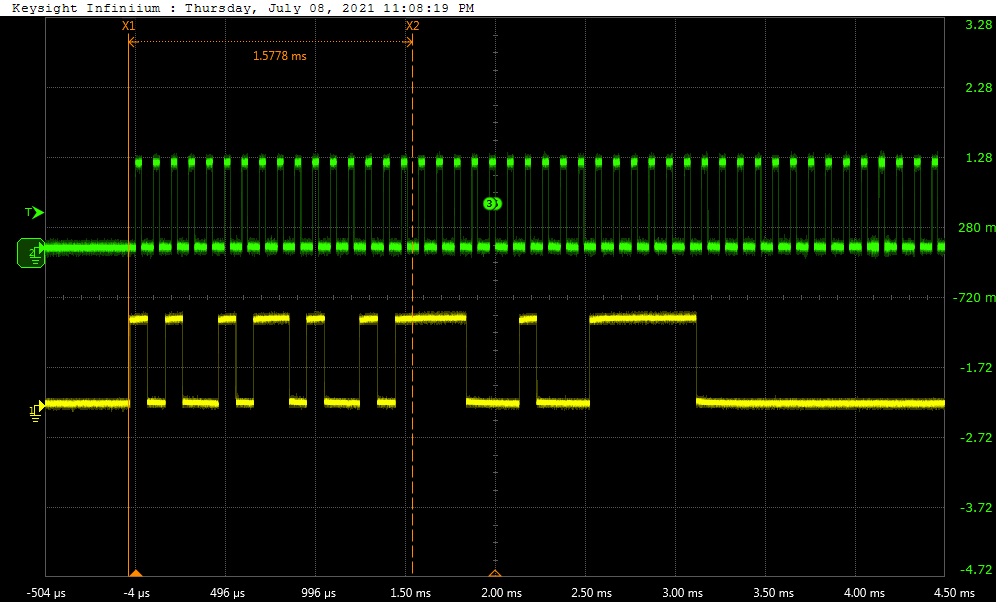
\includegraphics[width=0.5 \textwidth]{IMG/probe/09-08-2021_ch17-write63-baselinedac1.png}
	\end{center}
	\end{frame}

	
	\begin{frame}
	\frametitle{Reading Baseline DACs}
	\begin{columns}
		\column{0.5 \textwidth}
		{\color{blue} Input}
		\begin{itemize}
			\item Initialization sequence = A5A5
			\item Command = 10 = read
			\item Address = 001010 = 00101-0 = channel 05
			\item Data    = 00000000
		\end{itemize}
		\column{0.5 \textwidth}
		{\color{blue} Output}
		\begin{itemize}
			\item 11 = read
			\item 001010 = 00101-0 = channel 05
			\item 00110101 = 53
		\end{itemize}
	\end{columns}
		\begin{center}
			{\color{green} clock signal}
			{\color{yellow} input data}
			{\color{red} output data 2.5V}
			{\color{blue} output data 1.2V}
			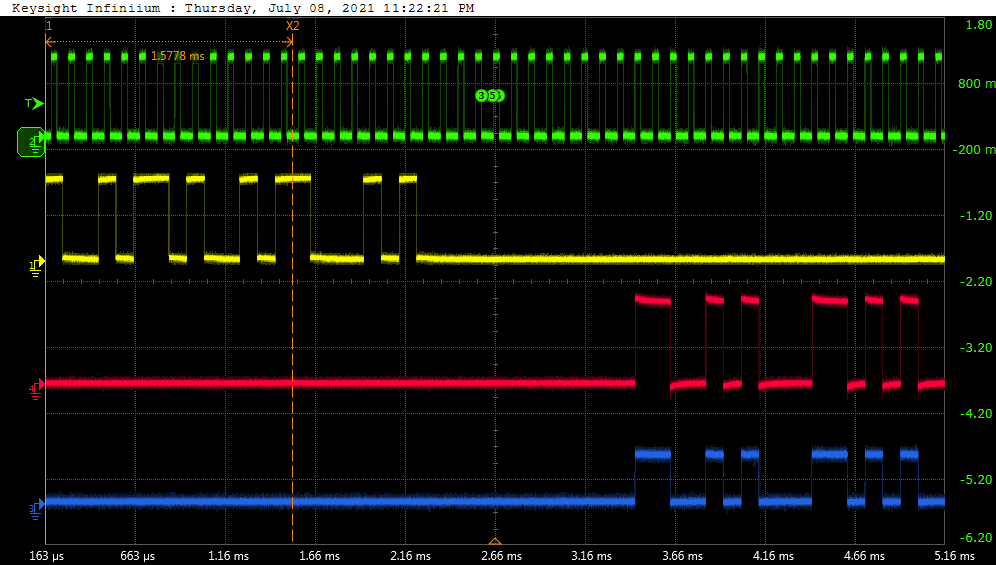
\includegraphics[width=0.5 \textwidth]{IMG/probe/09-08-2021_ch05-read53-baselinedac1.png}
		\end{center}
	\end{frame}

%%%%%%%%%%%%%%%%%%%%%%%%%%%%%%%%%%%%%%%%%%%%%%%%%%%%%%%%%%%%%%%%%%%%%%%%%%%%%%%%%%%%%%%%



	\section{Results}
	
	\begin{frame}[plain, noframenumbering]
	%\frametitle{results}
	\begin{center}
		{\Huge \fontfamily{qtm}\selectfont \color{blue} \textbf{Results}}
	\end{center}
	\end{frame}
	
	\begin{frame}
	\frametitle{threshold scan}
		\begin{itemize}
			\item Channel 1 threshold scan with \textbf{600}mV \textbf{10}KHz impulses
			\item {\color{blue}Blue} curve with baseline dac=\textbf{0}
			\item {\color{green}Green} curve with baseline dac=\textbf{63}  
		\end{itemize}	
		\begin{center}
			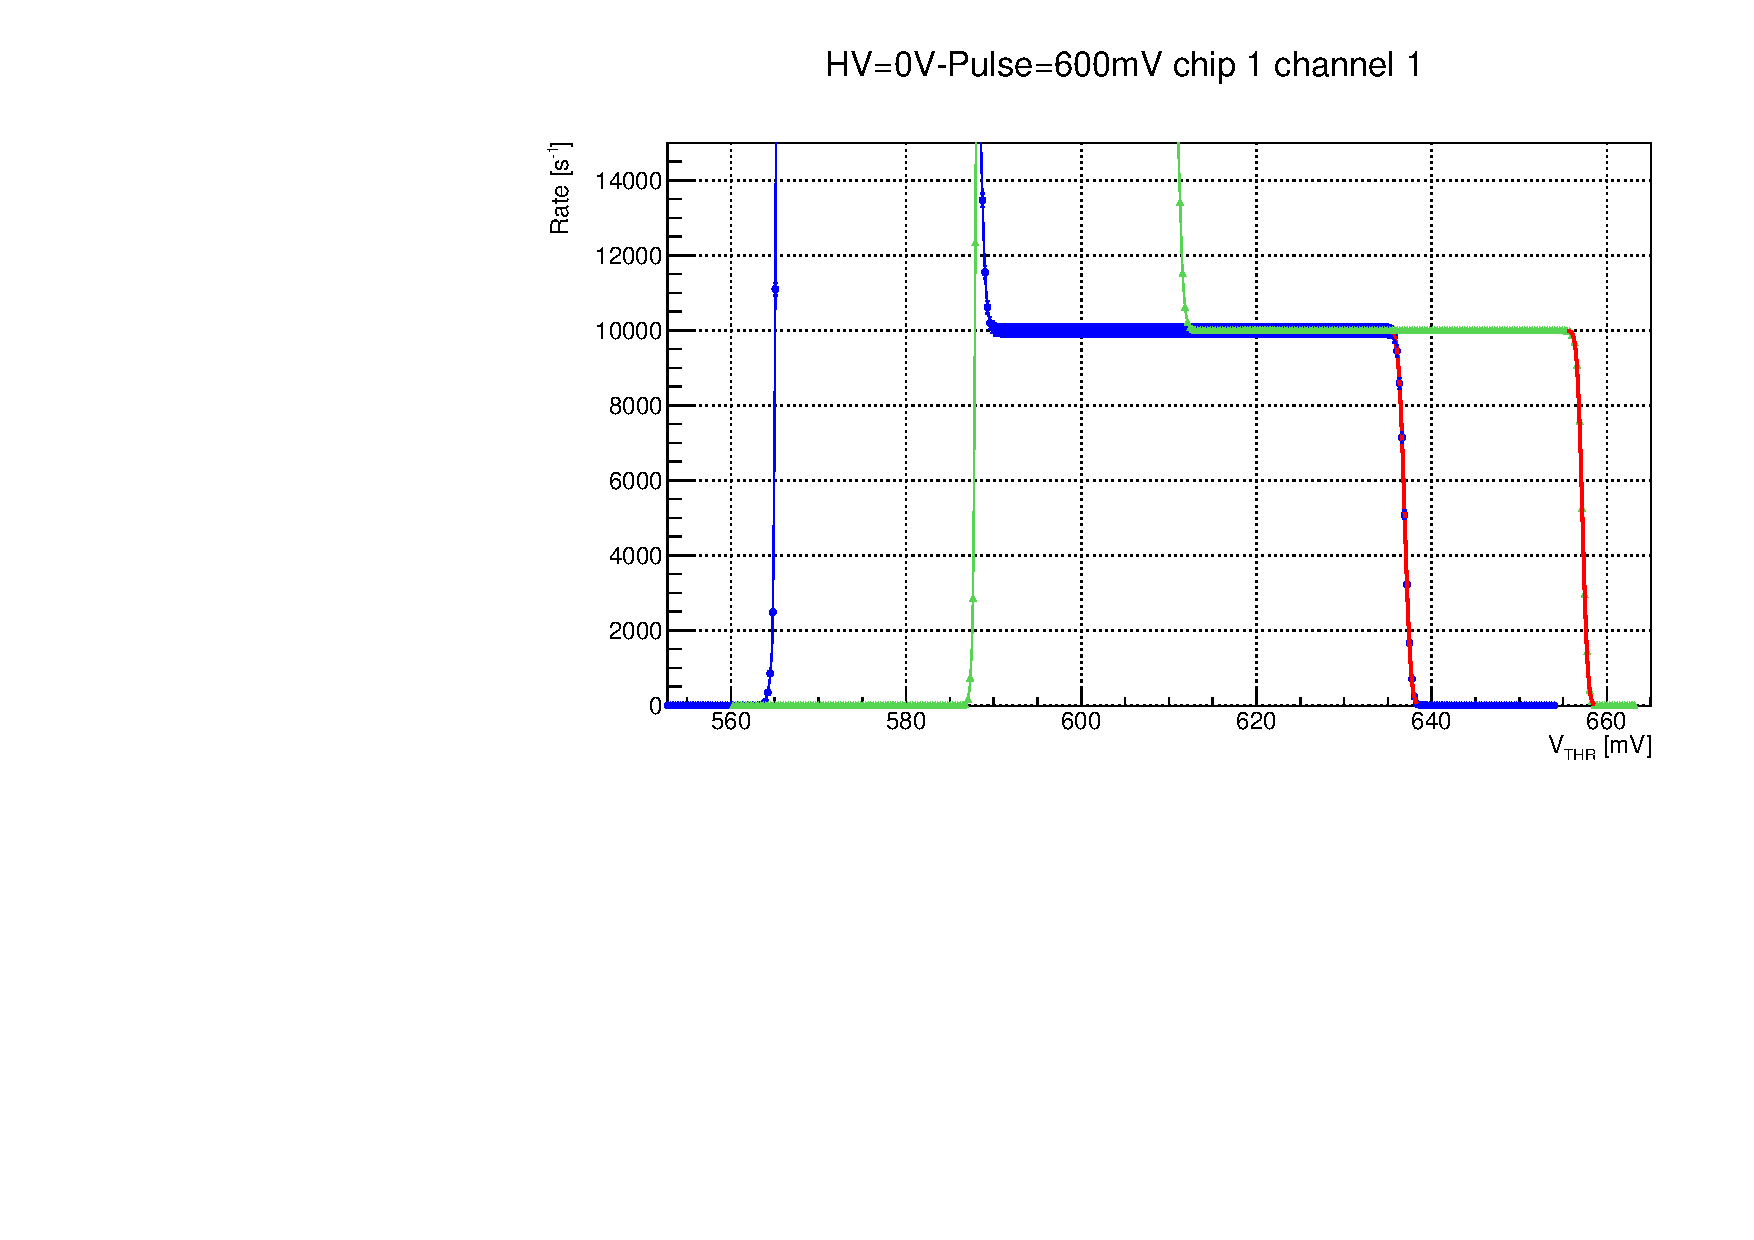
\includegraphics[width=0.65 \textwidth]{IMG/ThScan_ch0.pdf}
		\end{center}
		
	\end{frame}

	\begin{frame}
	\frametitle{Pedestal distribution}
	\begin{itemize}
		\item Pedestal voltage value for odd channels
		\item {\color{blue}Blue} dots with baseline dac=\textbf{0}
		\item {\color{red}Red} dots with baseline dac=\textbf{63}
	\end{itemize}
	\begin{center}
		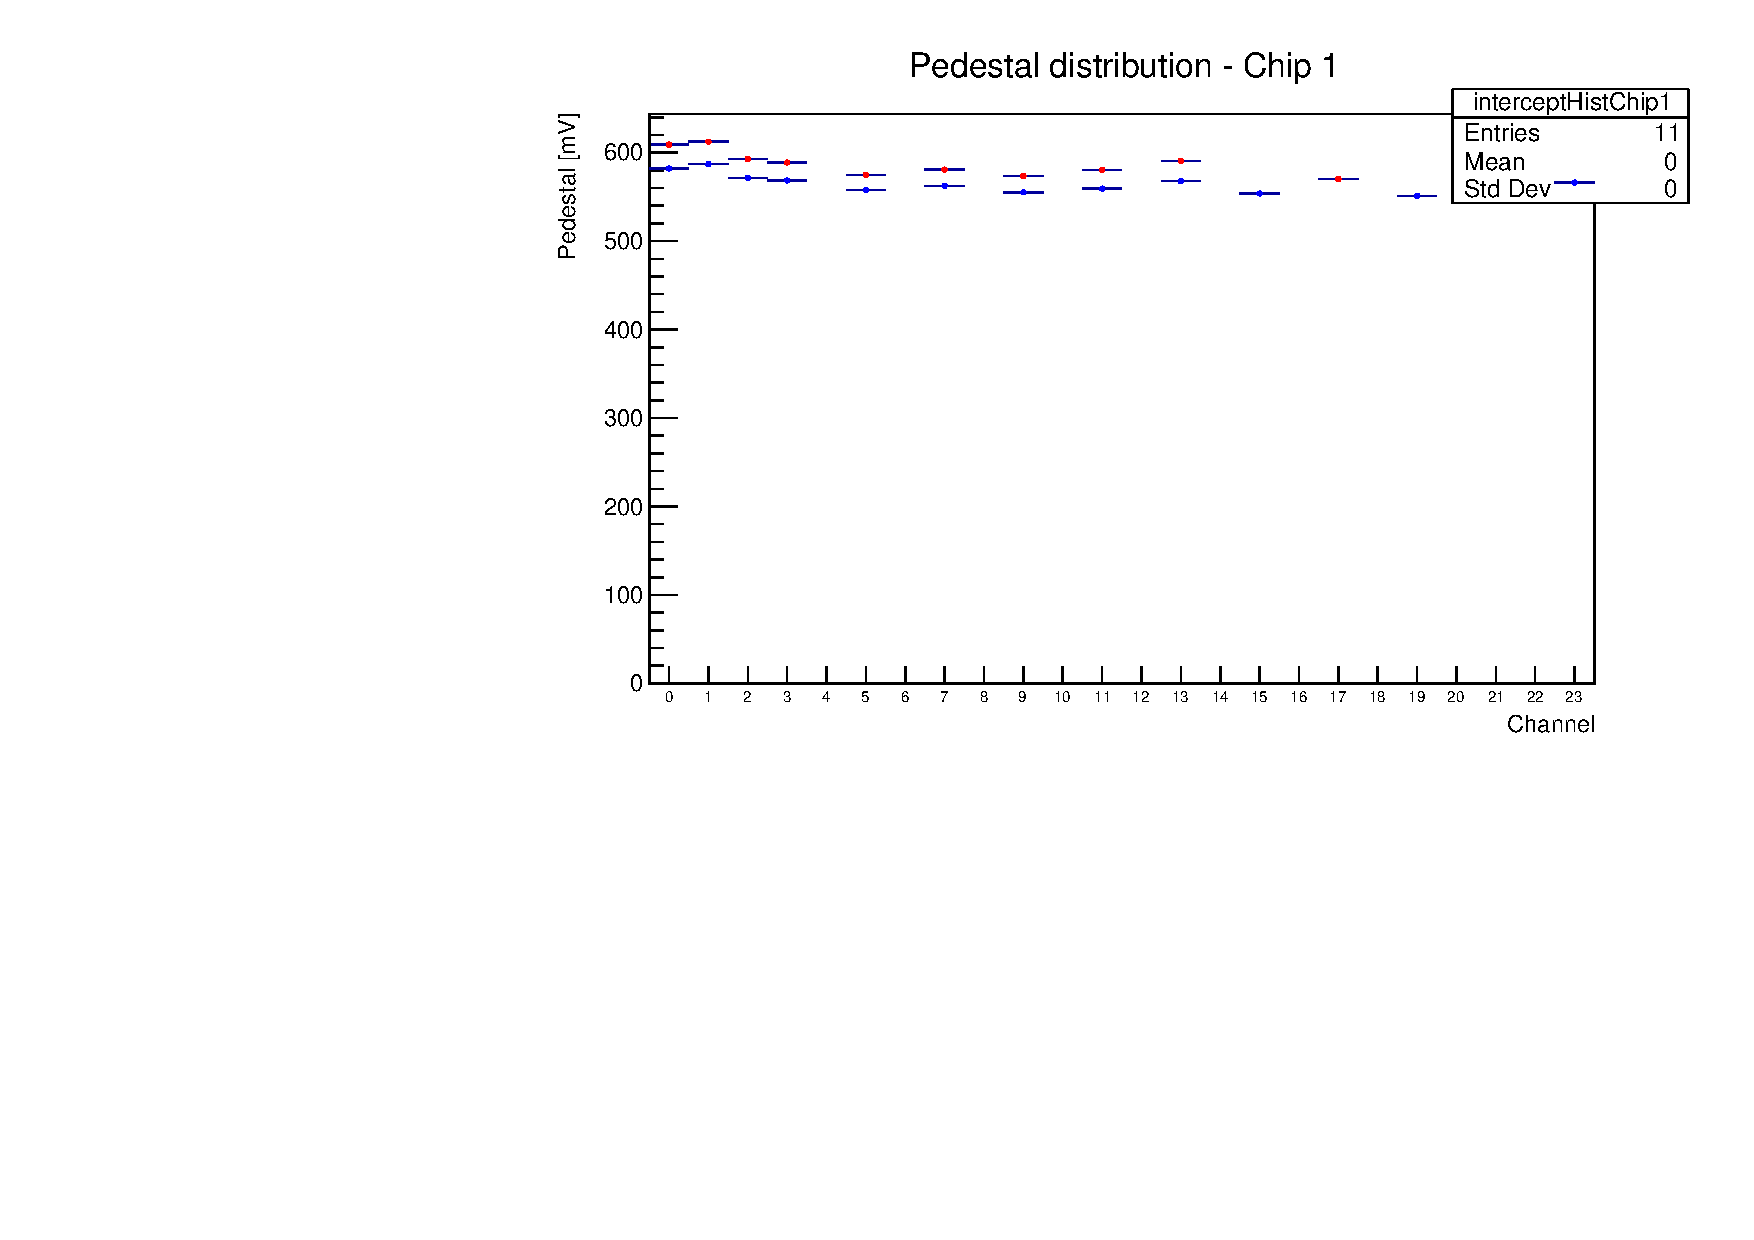
\includegraphics[width=0.65 \textwidth]{IMG/TB1-DAC0-DAC63.pdf}
	\end{center}
	
	\end{frame}

%%%%%%%%%%%%%%%%%%%%%%%%%%%%%%%%%%%%%%%%%%%%%%%%%%%%%%%%%%%%%%%%%%%%%%%%%%%%%%%%%%%%%%%%
	\section{Conclusions}
	
	\begin{frame}
	\frametitle{Conclusions }
	\begin{center}
		{\color{blue}\textbf{Future additions to the FPGA firmware}}
	\end{center}
		\begin{itemize}
			\item DACs \textbf{characterization} and verification of their \textbf{linearity}
			\item Addition of a \textbf{latch} in order to save into a \textbf{register} the current state of every counter 
			\item Addition of a \textbf{timestamp} in order to obtain a more accurate rate calculation 
			\item Addition of a configurable \textbf{mask} to calculate via firmware the \textbf{sum} of only certain selected channels 		
		\end{itemize}
			\vspace{1 cm}
		\begin{center}
			\textbf{Thanks for the attention!!}
		\end{center}	
	\end{frame}

	\begin{frame}[noframenumbering]
	\frametitle{Bibliography}
	{\scriptsize 
	\begin{thebibliography}{00}
		\bibitem{1}www.researchgate.net/figure/Dose-depth-curve-for-monoenergetic-photons-protons-and-carbon-ions-courtesy-of-GSI\textunderscore fig1\textunderscore283521369
		\newline
		\bibitem{2}www.intechopen.com/books/novel-prospects-in-oxidative-and-nitrosative-stress/oxidative-stress-in-hadrontherapy
		\newline
		\bibitem{3}www.semanticscholar.org/paper/A-Millimeter-Scale-Single-Charged-Particle-for-Lee-Scholey/ae955a07a42e9c124a8473357cd485b0b9928090
		\newline
		\bibitem{4}www.semanticscholar.org/paper/Low-Gain-Avalanche-Detectors-(LGAD)-for-particle-Moffat-Bates/0477d7bc2c9a3b26ad776874598f56d7d5b54c45
		\newline
		\bibitem{5}MoveIt v2 design document, Giovanni Mazza, January 15, 2021
	\end{thebibliography} }
	\end{frame}

%%%%%%%%%%%%%%%%%%%%%%%%%%%%%%%%%%%%%%%%%%%%%%%%%%%%%%%%%%%%%%%%%%%%%%%%%%%%%%%%%%%%%%%%
	\section{Backup}
	
	\begin{frame}[plain, noframenumbering]
	\begin{center}
		{\Huge \fontfamily{qtm}\selectfont \color{blue} \textbf{Backup}}
	\end{center}
	\end{frame}
	
	\begin{frame}[noframenumbering]
	\frametitle{Additional Graphs}
	\begin{columns}
		\column{0.3 \textwidth}
		\begin{center}
			\begin{figure}
				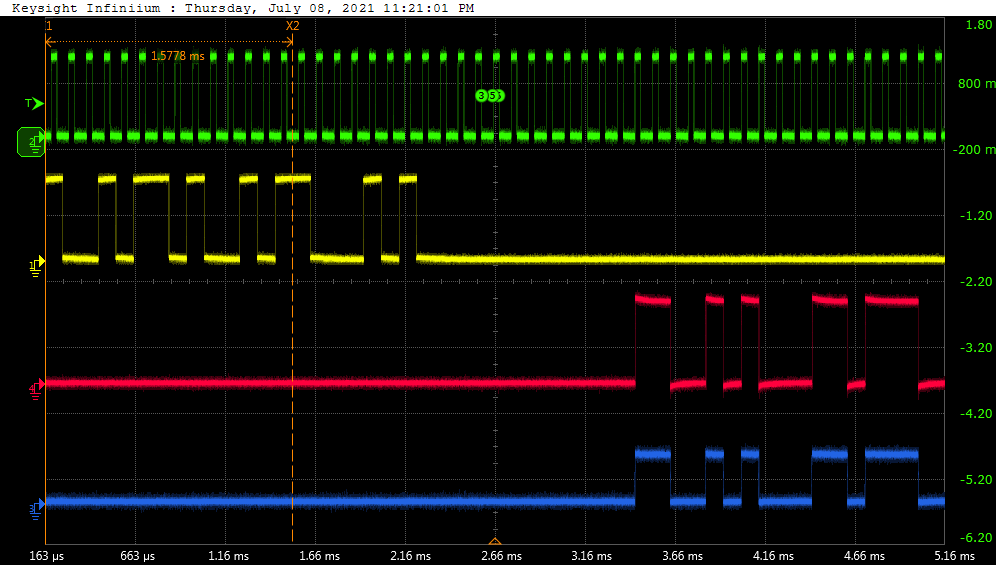
\includegraphics[width=0.95 \textwidth]{IMG/probe/09-08-2021_ch05-read55-baselinedac1.png}
				\caption{\centering{\tiny ch05-read55}}
			\end{figure}
			\begin{figure}
				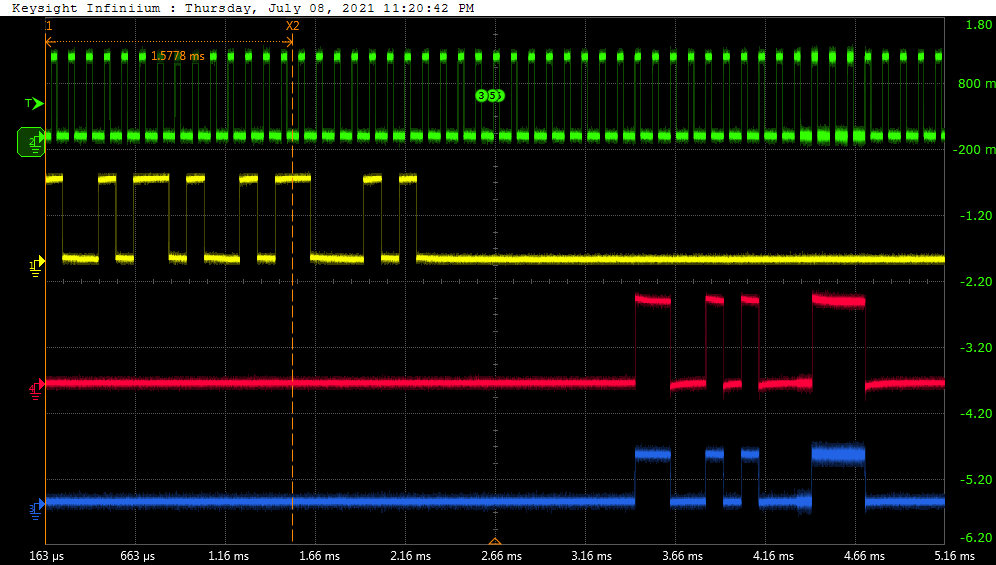
\includegraphics[width=0.95 \textwidth]{IMG/probe/09-08-2021_ch05-read56-baselinedac1.png}
				\caption{\centering{\tiny ch05-read56}}
			\end{figure}		
		\end{center}
		\column{0.3 \textwidth}
		\begin{center}
			\begin{figure}
				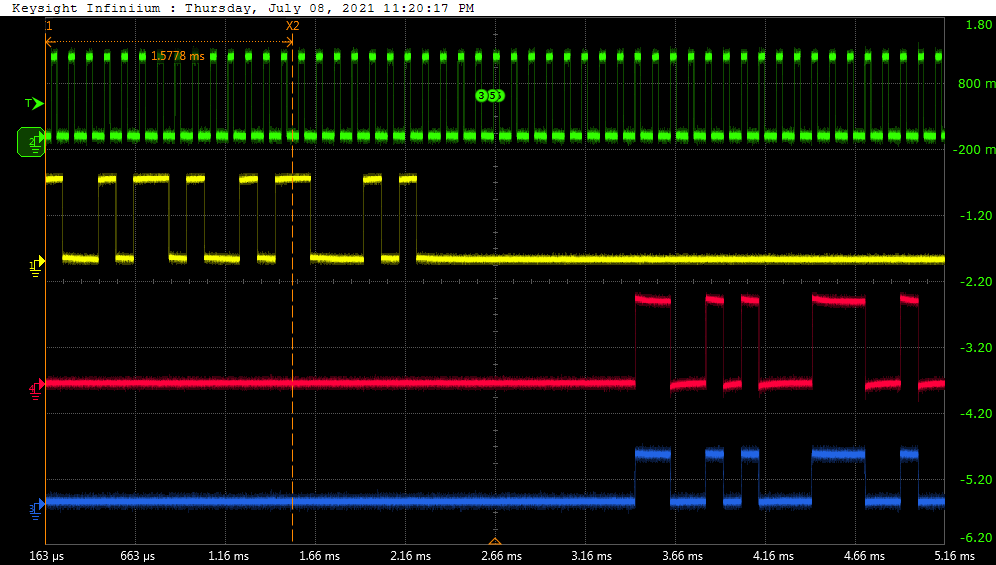
\includegraphics[width=0.95 \textwidth]{IMG/probe/09-08-2021_ch05-read57-baselinedac1.png}
				\caption{\centering{\tiny ch07-read57}}
			\end{figure}
			\begin{figure}
				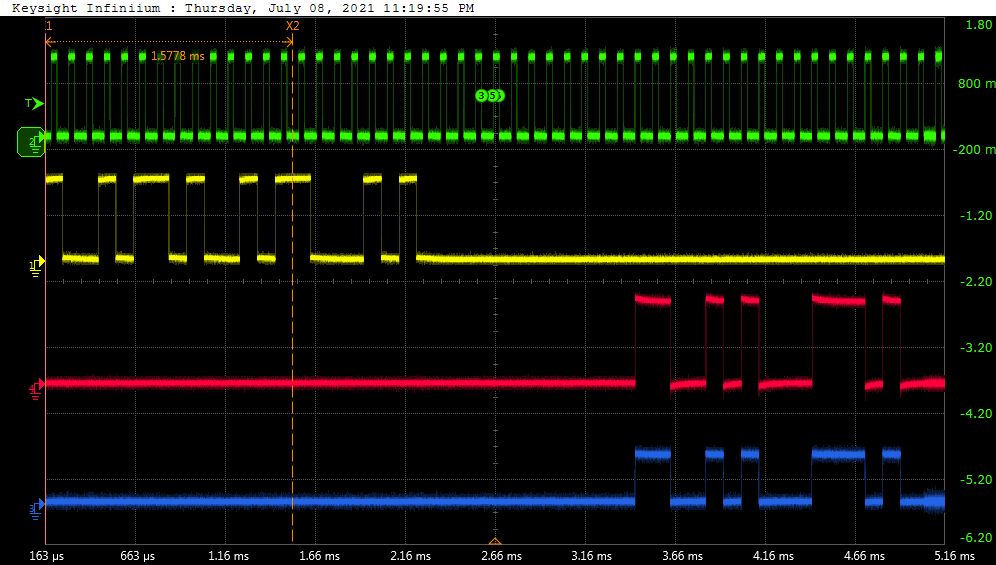
\includegraphics[width=0.95 \textwidth]{IMG/probe/09-08-2021_ch05-read58-baselinedac1.png}
				\caption{\centering{\tiny ch07-read58}}
			\end{figure}	
		\end{center}
		\column{0.3 \textwidth}
		\begin{center}
			\begin{figure}
				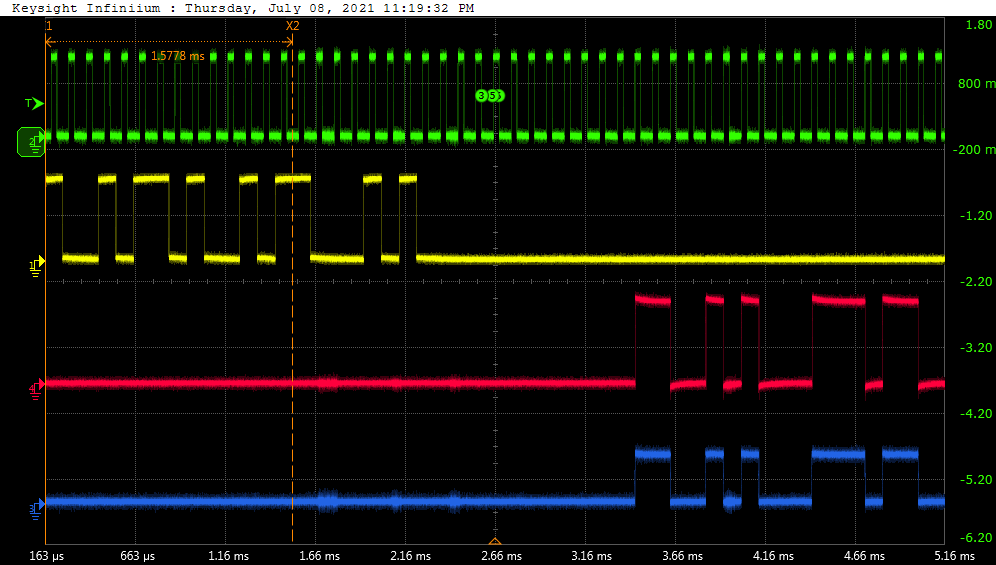
\includegraphics[width=0.95 \textwidth]{IMG/probe/09-08-2021_ch05-read59-baselinedac1.png}
				\caption{\centering{\tiny ch07-read59}}
			\end{figure}
			\begin{figure}
				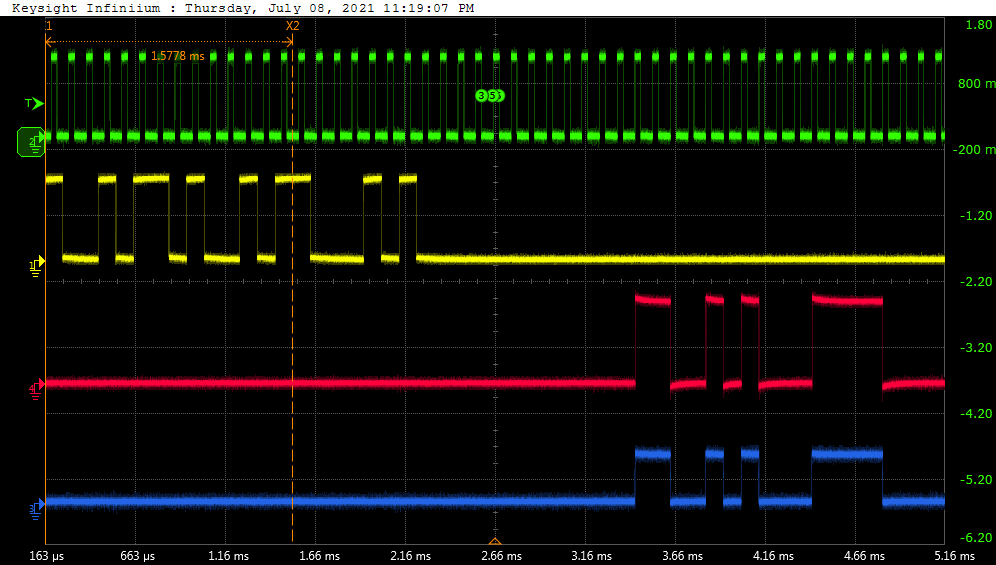
\includegraphics[width=0.95 \textwidth]{IMG/probe/09-08-2021_ch05-read60-baselinedac1.png}
				\caption{\centering{\tiny ch07-read60}}
			\end{figure}	
		\end{center}
	\end{columns}
		\end{frame}
	
	\begin{frame}[noframenumbering]
		\frametitle{I2C}
	\end{frame}

	\begin{frame}[noframenumbering]
		\frametitle{CML}
	\end{frame}

	\begin{frame}[noframenumbering]
		\frametitle{LVDS}
	\end{frame}

	\begin{frame}[noframenumbering]
		\frametitle{Constraints}
	\end{frame}

	\begin{frame}[noframenumbering]
		\frametitle{UDP}
	\end{frame}

	\begin{frame}[noframenumbering]
	\frametitle{Reading Baseline DACs $\rightarrow$ code}
	\begin{itemize}
		\item \textbf{reading} procedure for 1 dac consist of \textbf{2 processes}=
		\begin{itemize}
			\item \textbf{16}bit shift register
			\item sequence detector 
		\end{itemize}
	\end{itemize}
	\begin{center}
		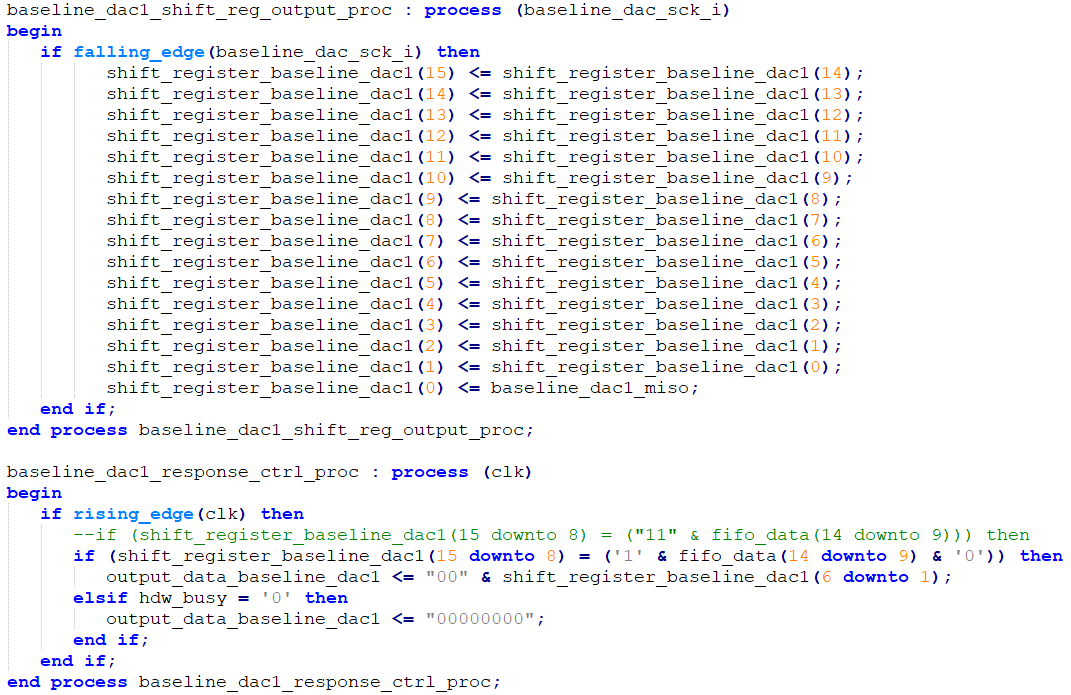
\includegraphics[width=0.6 \textwidth]{IMG/FSM_Read_States.png}
	\end{center}
	\end{frame}

		\begin{frame}[noframenumbering]
	\frametitle{VHDL}
	{\LARGE
		\begin{itemize}
			\item \textbf{VHDL}: \textbf{V}HSIC \textbf{H}ardware \textbf{D}escription \textbf{L}anguage 
			\begin{itemize}
				\item \textbf{VHSIC}: \textbf{V}ery \textbf{H}igh \textbf{S}peed \textbf{I}ntegrated \textbf{C}ircuits
				\item Is a hardware description language (\textbf{HDL}) that can model the behavior and structure of digital systems at multiple levels of abstraction
				\item Since \textbf{1987}, VHDL has been standardized by the Institute of Electrical and Electronics Engineers (\textbf{IEEE})
				\item In February 2008, Accellera approved \textbf{VHDL 4.0}, also informally known as VHDL 2008
				\item {\color{orange} VHDL is not a programming language!}
			\end{itemize}
		\end{itemize}
	}
\end{frame}
	
\end{document}